\documentclass[12pt,a4paper,bibtotoc,pointlessnumbers]{scrartcl}
\usepackage[ngerman]{babel}
%\usepackage[german]{polyglossia}
%\selectlanguage{german}
% ##########################################
% PDFLaTeX oder nicht:
\newif \ifPDF                                   
\ifx \pdfoutput \undifined \PDFfalse 
\else \ifnum \pdfoutput >0 \PDFtrue
     \else \PDFfalse         
     \fi     
\fi 
% ##########################################
\usepackage{lmodern} %ersetzt Standarsschrift --> für schönere Textdarstellung im PDF
\usepackage[onehalfspacing]{setspace} %setzt das Dokument in 1,5-fachem Zeilenabstand
\setlength\parindent{0pt}% Setzt den Einzug nach einem Absatz fest (hier auf Null)
\usepackage{microtype}

%\usepackage{csquotes}
%\usepackage[style=acm]{biblatex}
%\addbibresource{Literaur.bib}
\usepackage{bibgerm}
%\usepackage{natbib}

\usepackage[
backend=biber,
style=numeric,
%-verb
sorting=none
]{biblatex}

\addbibresource{BA-JannesBrunner.bib}
%\addbibresource{Bildquellen.bib}
%%\bibliography{Masterarbeit.bib}
%\usepackage{cite}
\DefineBibliographyStrings{ngerman}{%
	urlseen = {Abruf vom}
}


\usepackage[T1]{fontenc} %für europäischen ASCII-Code (mit Umlauten etc)
\usepackage[utf8]{inputenc} %Legt den Zeichencode fest

\usepackage[babel, german=quotes]{csquotes}

\usepackage[dvips]{graphicx} %damit Bilder eingebunden werden Können
\usepackage{fancyhdr} %Nachfolger zu "fancyheadings" --> legt Layout der Seite fest + hält zusätzliche Befehle und Optionen bereit

%\usepackage[headsepline]{scrlayer-scrpage}
%\automark[section]{subsection}

\usepackage{float} %Objekte, die nicht auf zwei Seiten aufgeteilt werden sollen (z.B. Bilder, Tabellen)
\usepackage{floatflt} %wird für die Umgebung floatfigure benötigt --> Bild kann von text umflossen werden
\usepackage[section]{placeins} %section verhindert, dass Bilder aus section hinausgleiten

\usepackage{amsmath} %für Matheumgebung
\usepackage{amssymb} %Setzt Befehle für Symbole in Symbole um 
\usepackage{amsfonts} %Zusätzliche Schriften und Symbole
\usepackage{exscale} %stellt Befehle für Änderung der Schrift bereit
\usepackage{textcomp}
\usepackage{easymat} % weitere Befehle für Matrizen
\usepackage{enumitem} % Ändern von Listenumgebungen
%\usepackage{paralist}

\usepackage{pdfpages}%erlaubt das einbinden von anderen PDF-Dokumenten (auch einzelnen Seiten) in das Latex-Dokument

\usepackage{etex} %erhöht die Anzahl der Pakete, die geladen werden können

\usepackage[font=small,labelfont=bf,hang]{caption} %für Bild- und Tabellenunterschriften
\addto\captionsngerman
{
	\renewcommand{\figurename}{\small{\textbf{Abb.}}}
	\captionsetup{figurewithin = section}
}
\addto\captionsngerman{
	\renewcommand{\tablename}{\small{Tab.}}}
\captionsetup{tablewithin = section}
\captionsetup{font=small, labelfont=bf}

\usepackage{listings} % für code listings
\definecolor{lightgray}{rgb}{.9,.9,.9}
\definecolor{darkgray}{rgb}{.4,.4,.4}
\definecolor{purple}{rgb}{0.65, 0.12, 0.82}

\lstdefinelanguage{JavaScript}{
	keywords={typeof, new, true, false, catch, function, return, null, catch, switch, var, const, let, if, in, while, do, else, case, break},
	keywordstyle=\color{blue}\bfseries,
	ndkeywords={class, export, boolean, throw, implements, import, this},
	ndkeywordstyle=\color{darkgray}\bfseries,
	identifierstyle=\color{black},
	sensitive=false,
	comment=[l]{//},
	morecomment=[s]{/*}{*/},
	commentstyle=\color{purple}\ttfamily,
	stringstyle=\color{red}\ttfamily,
	morestring=[b]',
	morestring=[b]"
}

\lstset{
	language=JavaScript,
	backgroundcolor=\color{lightgray},
	extendedchars=true,
	basicstyle=\footnotesize\ttfamily,
	showstringspaces=false,
	showspaces=false,
	numbers=left,
	numberstyle=\footnotesize,
	numbersep=9pt,
	tabsize=2,
	breaklines=true,
	showtabs=false,
	captionpos=b
}

\lstdefinestyle{tinyListing}{
	language=Matlab,
	numbers=left,
	stepnumber=1,
	numbersep=10pt,
	tabsize=4,
	showspaces=false,
	showstringspaces=false
}

%\usepackage{subfig}
\usepackage{subcaption}
\usepackage{longtable}% erlaubt Tabellen über mehrere Seiten
\usepackage{tabularx} %Tabellen können größer gemacht werden und und die Spalten sind flexibler
\renewcommand\tabularxcolumn[1]{m{#1}}% for vertical centering text in X column
\usepackage{booktabs} %definiert Befehle für Tabellen
%\usepackage{booktabs-de}
\usepackage{ltxtable} %vereinigt longtable und tabularx
\usepackage{tabu} %verbesserte ltxtable ?
\usepackage{colortbl}
\usepackage{multirow}
%\usepackage{multicolumn}
\usepackage{rotating}
%\usepackage{tablefootnote}
%\usepackage{filecontents} % Es besteht die Möglichkeit eine ltxtable Tabelle direkt innerhalb des Dokumentes zu setzten.
%\usepackage{tikz}

\usepackage{array} %erweiterte Möglichkeiten für Tabellen und Spalten
%\usepackage{subfigure}
\usepackage{url} %lange Zeichenfolgen können trotz fehlender Leerzeichen getrennt werden
%\usepackage{paralist}
% ##########################################

% ##########################################
% Seitendesign:
\usepackage{units}
\usepackage[headheight=50pt, a4paper, bottom=25mm, footskip=6mm]{geometry} %wird für Layout des Dokuments benötigt
\geometry{verbose}
% ##########################################
%\usepackage{cite} % fasst Zitate zusammen (funktioniert nur ohne hyperref)

\ifPDF
\usepackage{xcolor}   %ermöglicht das Ändern der Farbe von Schrift, Seitenhintergrund, Boxen etc
\usepackage[
  pdftex,
  colorlinks,
  citecolor = {green},
  linkcolor = {black},
  urlcolor  = {gray},                
  bookmarks         = true,
  bookmarksopen     = true, % Bookmarks anzeigen...
  bookmarksnumbered = true, % ...und numerieren
  pdftitle          = {BA},
  pdfauthor         = {Jannes Brunner}
]{hyperref} %ermöglicht Links im PDF-Dokument (z.B. ancklicken eines Kapitel im Inhaltsverzeichnis oder Verlinkung mit externem Link)


\else
\usepackage{wrapfig}
%\usepackage{floatflt} %ermöglicht Gleitobjekte (Bilder, Tabellen) von Text umfließen zu lassen und Bilder links/recht je nach Seitenzahl auszurichten
\fi%-----------------------------------------------------------------------------
% Definition für einen neuen Befehl für deutsche Anführungszeichen
\newcommand{\gqq}[1]{\glqq{}#1\grqq{}}
\newcommand{\gq}[1]{\glq{}#1\grq{}}


\begin{document}
	\begin{titlepage}
		\begin{center}
%				\begin{figure}[h]
%					\begin{minipage}{.4\textwidth}
%						\centering
%						\includegraphics[width=0.5\textwidth]{Bilder/Logo_Wildau}
%					\end{minipage}
%					\begin{minipage}{.2\textwidth}
%						\hspace{\textwidth}
%					\end{minipage}
%					\begin{minipage}{.4\textwidth}
%						\centering
%						\includegraphics[width=0.4\textwidth]{Bilder/bam_logo_135}
%					\end{minipage}
%				\end{figure}			
%				\vspace{0.4cm}
			
%			{\large \bf Bundesanstalt für Materialforschung und -prüfung }\\[4mm]
%			{\large\bf TH Wildau}
			%\vspace{0.5cm} \hrule \vspace{1.3cm}
			
			 
			\begin{doublespace}
			{\huge Entwicklung einer webbasierten Client-Server Anwendung zur Unterstützung von interaktiven Unterrichtsmethoden}\\
			\end{doublespace}
			\vspace{2cm}
			{\huge \bf Bachelorarbeit}\\
			\vspace{0.4cm}
			
			{\large zur Erlangung des akademischen Grades\\ Bachelor of Science \\ an der HTW Berlin}\\
			
			\vspace{1cm}
			
			{\Large \bf Hochschule für Technik und Wirtschaft Berlin}\\
			{\large \bf Fachbereich Informatik, Kommunikation und Wirtschaft\\
			internationaler	Studiengang Medieninformatik}\\
		
			\vspace{1.5cm}
			
			{\doublespacing Eingereicht von\\
			{\Large \bf Jannes Julian Brunner}\\ geb. 21.06.1991}
			
%			\vspace{1cm}
		
			\large
			\begin{table}[b]
				\begin{center}
					\begin{tabular}{ll}
					Eingereicht am:& 05.08.2019\\
					Betreuender Hochschuldozent:& Prof. Dr. Gefei Zhang\\
					Zweitgutachter: & Prof. Dr.-Ing. Kai Uwe Barthel\\
					\end{tabular}
				\end{center}
			\end{table} 
		\end{center}
		\vspace{0.6cm}
	%	{\bf Abstract}: Das Abstract
\end{titlepage}

\newpage
%\clearpairofpagestyles




%\clearpairofpagestyles

\pagenumbering{roman}
\setcounter{page}{2}

\thispagestyle{empty}
\section*{Abstract}\label{sec:abstract}
\newpage

%\thispagestyle{empty}
\cfoot{\pagemark}
\tableofcontents
\newpage

\pagenumbering{arabic}




%\pagestyle{scrheadings}
%\ihead{\leftmark}
%%\automark{section}
%\chead{\rightmark}
%%\automark{subsection}
%\ohead{\thepage}


\pagestyle{fancy}
\fancyhf{}
%\setlength{\headheight}{15pt}
\renewcommand{\headrulewidth}{0.4pt} %definiert die Dicke der Linie unter der Kopfzeile
%\renewcommand{\footrulewidth}{0pt} %definiert die Dicke der Linie über der Fußzeile
\renewcommand{\sectionmark}[1]{%
	\markboth{\thesection.\ #1}{}} %sorgt dafüpr, dass die Kapitel und Unterkapitel in der Kopfzeile stehen


%\addtolength{\headwidth}{\marginparwidth}
%\setlength{\fancyhead}{0.4\headrulewidth}
\fancyhead[L]{\textsl{\small 
%		\leftmark \hspace{0.8cm}
		\rightmark}}
%\fancyhead[C]{\parbox{0.5\textwidth}{\textsl{\small \rightmark}}}
\fancyhead[R]{\textsl{\small \thepage}}
%\fancyhead[L]{\parbox{0.3\textwidth}{\textsl{\small \leftmark}}}
%\fancyhead[C]{\parbox{0.6\textwidth}{\textsl{\small \rightmark}}}
%\fancyhead[R]{\parbox{0.05\textwidth}{\textsl{\small \thepage}}}
%\addtolength{\headwidth}{\marginparsep}
%\fancyfoot[C]{\thepage}


\section*{Fachbegriffe und Formelzeichen}
\addcontentsline{toc}{section}{Fachbegriffe und Formelzeichen}
%\begin{center}
%	\textbf{Begriffe und Formelzeichen}
%\end{center}
\begin{longtable}{llp{6.5cm}}
	\textbf{Parameter} & \textbf{Formel-} & \textbf{Einheit/Beschreibung}\\
	 & \textbf{zeichen} & \\
	Abschirmkonstante & $ S_n $ & Gibt die Abschirmung von Elektronen auf äußeren Energieniveaus in Atomen mit mehreren Elektronen an\\
	Absolute Temperatur & T & in Kelvin (K)\\ 
\end{longtable}

\vspace{1cm}

%\begin{center}
%	\textbf{Abkürzungen}
%\end{center}

\section*{Abkürzungsverzeichnis}
%\twocolumn[\centering\textbf{Abkürzungen}]
\addcontentsline{toc}{section}{Abkürzungsverzeichnis}

\begin{tabularx}{0.9\columnwidth}{lX}
	AJAX & Asynchronous JavaScript and XML \\
	DARPA & Defense Advanced Research Projects Agency\\
	ARPANET & Advanced Research Projects\\
	WWW & World Wide Web \\
	LAN & Local Area Network \\
	WLAN & Wireless Local Area Network \\
	WAF & Web-Application-Framework \\
\end{tabularx}



%\onecolumn
	
%\begin{minipage}[H]{0.5\textwidth}
%		\begin{center}
%		\textbf{Abkürzungen}
%	\end{center}
%	\begin{tabularx}{\textwidth}{ll|}
%		RFA & Röntgen Fluoreszenz Analyse\\
%		XRF & X-ray fluorescence analysis (siehe: RFA)
%	\end{tabularx}
%\end{minipage}
%\begin{minipage}[H]{0.5\textwidth}
%
%\end{minipage}
\newpage

\section{Einführung}\label{sec:einfuhrung}
\subsection{Motivation}\label{sec:motivation}

Bildung ist ein wichtiges Element der Persönlichkeitsentwicklung und unter Artikel 26 der allgemeinen Erklärung der Menschenrechte als solches definiert. Ohne Bildung ist das Ausüben eines gewählten Berufes und das Entwickeln einer Meinung zu komplexen Sachverhalten unmöglich. \cite{weitblicker.org2019:online}. Heute sieht sich Bildung durch den digitalen Wandel der letzten Jahre sich noch nie vorher dagewesenen Problemen gegenübergestellt. Wie können Lehrende an Schulen digitale Technik effizient und preiswert im Unterricht einsetzen und so neue Bildungskonzepte erfolgreich in den Lehrplan integrieren? Ursprünglich bezeichnet der Begriff Digitalisierung das Umwandeln von Analog nach Digital. Wurde früher Musik auf Schallplatten vertrieben, so wurde diese von der Compact Disc vom Markt verdrängt, welche die Musik auf kleinerem Raum digital abspeichert. Auch wenn der Begriff im Zusammenhang mit Schule längst nicht mehr das Ursprüngliche meint, halte ich es für sehr wichtig, früher dagewesene Unterrichtskonzepte nicht einfach zu digitalisieren sondern es erfordert ein Neudenken. Bewährte pädagogische Methoden sollten durch Digitalisierung profitieren sowie neue Konzepte müssen erforscht und entwickelt werden. 

\subsubsection{Besuch Grundschule am Rüdesheimer Platz Berlin}\label{sec:grundschulebesuch}
Im Rahmen der Vorrecherche zu dieser Arbeit wurde einem Unterrichtstag in 
einer Jahrgangsübergreifenden (JüL) Klasse 1 bis 3 an der Grundschule am Rüdesheimer Platz beigewohnt um ein differenzierteres 
Bild der gegenwärtigen Lern- und Digitalisierungssituation an einer Berliner Schule zu bekommen. An dieser Stelle eine große Dankaussagung an Frau Wewer, Grundschullehrerin, welche diese Erfahrung möglich gemacht hat und in einem anschließenden Gespräch das Interesse an einer kostengünstigen und einfach nutzbaren Lösung zur Unterstützung von interaktiven Unterrichtsmethoden unterstrichen hat.
\newpage
\subsection{Problemstellung}\label{sec:problemstellung}
%Kurze Zusammenfassung des Forschungsstandes genügend?
Am 04.04.2019 trat die Änderung des Art. 104c des Grundgesetz für die Bundesrepublik Deutschland in Kraft
und ebnete so den Weg für den von Bund und Ländern beschlossenen Digitalpakt Schule \cite{Art104cG55:online}. 
Dieser Beschluss macht deutlich, dass digitale Kompetenz im Bildungssektor von hoher Bedeutung ist, was auch von einer Förderungssumme von mindestens 5,5 Milliarden Euro unterstrichen wird. 
Legt man diese Summe auf die ca 40.000 Schulen um, erhält jede Schule einen Durchschnittsbeitrag von 137.000 Euro. Bei ca. 11 Millionen Schülerinnen und Schülern würde das eine Förderungssumme von ca. 500 Euro pro Schülerin bzw. Schüler bedeuten. 
Einer der Hauptförderungspunkte des Digitalpakt Schule sieht den Ausbau der technischen Infrastruktur
an deutschen Schulen vor, z.B. Bereitstellung von drahtlosen Netzwerken, schnellen Internetzugangspunkten und digitale Unterrichtsmedien wie interaktive Whiteboards.
\\ \\
Das Bundesministerium für Bildung und Forschung (BMBF) gegenargumentiert damit, dass kein digitales Medium alleine gute Bildung fördert, sondern immer dahinterstehende pädagogische Konzepte aus einer Vielfalt von Angeboten entscheidend sind. \cite{dpakt2019:online} Ergänzend dazu kritisiert Dennis Horn (Experte für digitale Themen der ARD) den zu starken Fokus auf Hardware und mahnt an, dass zu wenig darüber gesprochen wurde, wie diese denn auch sinnvoll genutzt werden kann.\cite{Horn2018:online}. \\ \\
Diese Kritikpunkte wurden auch auf der Podiumsdiskussion der re:publica 2018 - 'Was kommt in den digitalen Schulranzen?' angeschnitten. Tobias Hübner, Lehrer und Autor im Bereich Medienistik, zeigt dort ebenfalls auf, dass der Wille Geld auszugeben zu begrüßen sei, es aber an Konzepten und Materialien mangele. Als Lehrer würde er den Investitionsfokus auf Lehrerfortbildung setzen.
\\ \\

Der populäre Tablet Computer 'iPad' der Firma Apple inc. kostet in der günstigsten Variante bereits mindestens 449€ \cite{iPadmini65:online} (Stand April 2019), was schon knapp 90\% des Förderungsvolumens pro Schülerin und Schüler ausmachen würde. Als ein Gegensatz wäre hier der Einplatinencomputer Raspberry Pi zu nennen, welcher bereits für 33 Euro erwerblich ist (Stand April 2019) und genug Rechenkapazitäten bereitstelle um zahlreiche Projekte im Bildungsbereich durchzuführen. Mit Touchscreenmodul und Schutzhülle liegt der Preis insgesamt bei ca. 150 Euro, was immer noch weniger als die Hälfte des Fördervolumens beträgt. 

\begin{figure}[H]
	\centering
	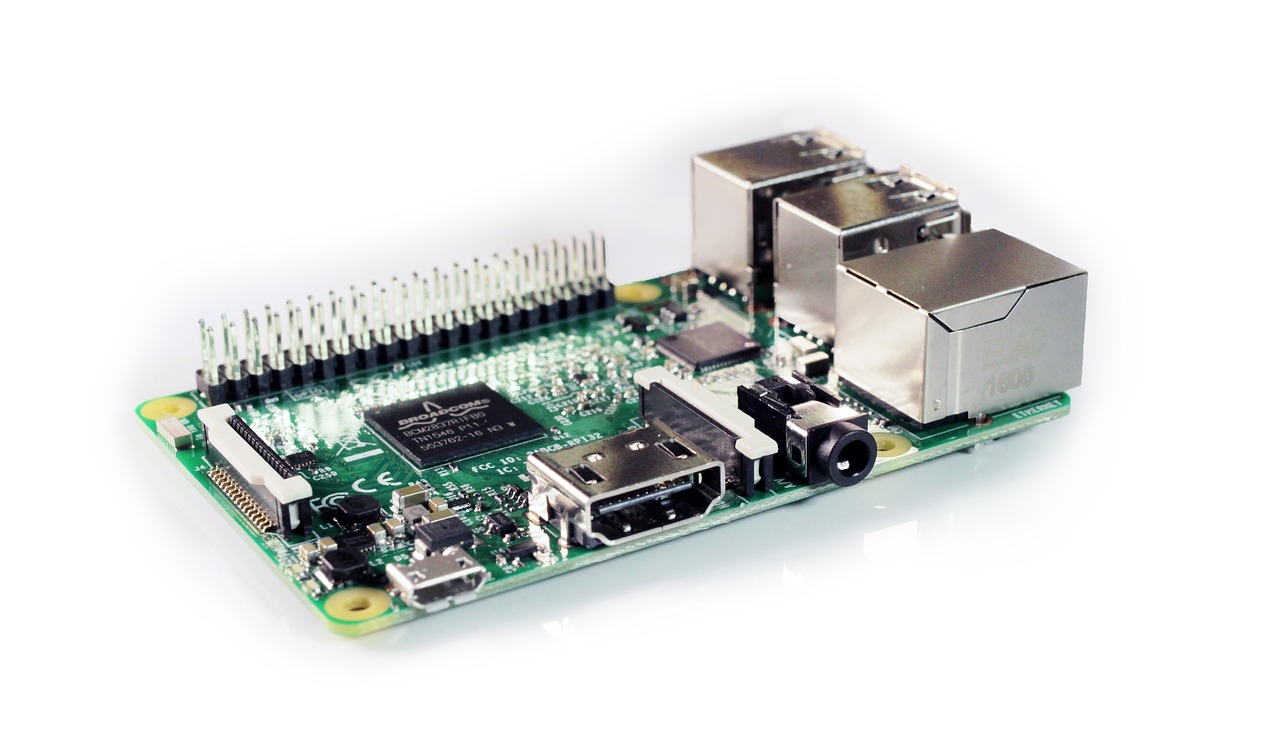
\includegraphics[width=0.8\linewidth]{bilder/raspberry-pi}
	\caption[Raspberry Pi 3 - Einplantinencomputer]{Der Raspberry Pi 3 - Einplantinencomputer \cite{PixaPi2016}}
	\label{fig:server_diagram}
\end{figure}


\subsection{Zielsetzung}\label{sec:zielsetzung}
Seit dem Erfolgskurs des Web 2.0\footnote{Web 2.0 ist ein Schlagwort, das für eine Reihe interaktiver und kollaborativer Elemente des Internets, speziell des World Wide Webs, verwendet wird. Dabei konsumiert der Nutzer nicht nur den Inhalt, er stellt als Prosument selbst Inhalte zur Verfügung. - Wikipedia.org} in den frühen 2000er Jahren, zeichnet sich zunehmend der Trend des Software-as-a-Service Geschäftsmodells ab. Dies beschreibt die Bereitstellung von Software im Internet oder durch ein lokal laufenden Servers, ohne dass Benutzende die Software selbst noch lokal installiert haben müssen. Im Jahr 2015 setzten bereits über drei Viertel von 102 befragten Unternehmen Software dieser Form aktiv im Geschäft ein\cite{TecArt-GmbH2019:online}. Viele Arten von Software können  mittlerweile in einer im Webbrowser lauffähigen Alternative substituiert werden. Ein populäres Beispiel ist die Office-Suite Google Docs der Firma Google inc. Hier lassen sich Textverarbeitung, Tabellenkalkulation und das erstellen von Präsentationen ohne Installation und direkt im Webbrowser des Benutzenden ausführen. Ein anderes Beispiel ist die Web-Software Photopea welche ebenfalls komplett im Web-Browser ausgeführt wird und dem nur lokal installiert ausführbaren quasi Industriestandard Bildbearbeitungsprogramm Photoshop der Firma Adobe inc. sehr nahe kommt. Im Vergleich zu lokal installierter Software ist die Bereitstellung von Web-Software einfacher, da solange ein moderner Webbrowser lauffähig ist, das Betriebssystem des Client-Computers zu vernachlässigen ist. Ebenso stellt potente Hardware keine zwingende Voraussetzungen, da etwaige rechenintensive Aufgaben auf der Serverseite getätigt werden können oder hier eine Balance zwischen Client und Server angestrebt werden kann. \\ 
% Das da oben noch Teil der Problemstellung?
%Hier jetzt Web Trend noch erwähnen!
Ein Raspberry Pi Einplantinencomputer bietet bereits genügend Leistung für Webtechnologien und ein günstigen Anschaffungspreis. Auch besitzen bereits 67\% der 10-11 jährigen Jugendlichen ein Smartphone \cite{Statista2017:online} welches ebenfalls genug Leistung für Webanwendungen aufweisen. \\ \\ Eine Softwarelösung zur Unterstützung von interaktiven Unterrichtsmethoden, welche auf Webtechnologien basiert, könnte den Rahmen der im Digitalpakt Schule fließenden Gelder optimierter ausschöpfen und Schulen finanzielle Flexibilität einräumen. 
\\ \\
Diese Arbeit wird sich der Thematik von pädagogischen digitalen Konzepten und Varianten von interaktiven Unterrichtsmethoden nur im Rahmen der Softwareentwicklung widmen und ihre forschungsrelevante Tiefe nicht gänzlich erfassen, da dies den Rahmen der Zielsetzung überschreiten würde.

%wichtigste Quellen hier noch nennen un
\newpage

\subsection{Aufbau der Arbeit}
Im Anschluss an dieses Kapitel werden \hyperref[sec:grundlagen]{\textbf{Grundlagen}} erörtert. Dies umfasst die Themengebiete Digitalisierung an Schulen und einen Überblick über Webtechnologie. Ersteres ist für den späteren potentiellen Einsatz der Software maßgebend, letzteres bildet das technologische Fundament, welches die Implementierung erst möglich macht. Anschließend wird in Kapitel \hyperref[sec:analyse]{\textbf{Analyse}} ein Vergleich zwischen existierenden kommerziellen und nicht-kommerziellen Plattformen gezogen. Darauf aufbauend folgt eine Anforderungs- und Systembeschreibung. Im darauffolgenden Kapitel \hyperref[sec:konzept]{ \textbf{Konzept}} wird ebendieses erörtert und darauffolgend der Prozess der \hyperref[sec:implementierung]{\textbf{Implementierung}} beschrieben. In einer folgenden \hyperref[sec:auswertung]{\textbf{Auswertung}} werden die Ergebnisse mit den geplanten Zielen verglichen und ein Fazit gezogen. Schlussendlich wird im letzten Abschnitt ein \hyperref[sec:ausblick]{\textbf{Ausblick}} formuliert, welcher die Zukunft des Projekts betrifft. 
   

\newpage

\section{Zielsetzung}\label{sec:zielsetzung}
%wichtigste Quellen hier noch nennen un
% - Hypothese formulieren  
% - Methode (Arbeitsschritte/Vorgehensweise) + wichtigste Quellen benennen 

Das Ziel der Arbeit ist es, eine auf Webtechnologien basierende Softwarelösung zur Unterstützung von interaktiven Unterrichtsmethoden zu entwickeln.

Dabei soll auch untersucht werden, ob eine gänzlich vom Internet unabhängige Lösung umsetzbar ist. Sollte keine ausreichende Netzwerkinfrastruktur vorhanden sein, soll diese von der Software selbst in Form eines drahtlosen Netzwerks eingerichtet und gestellt werden. Dies könnte 
Schulen mit langsamer oder gar nicht vorhandene Internetanbindung und Netzwerkinfrastruktur den Einsatz von 
digital gestützten Unterrichtsmethoden erleichtern. 
\\ \\
Darauf aufbauend sollen die Mindesthardwareanforderungen gering gehalten werden. 
Ein niedriger Einrichtungspreis könnte den Rahmen der im \emph{Digitalpakt Schule} fließenden Gelder effizienter ausschöpfen und Schulen mehr finanzielle Flexibilität einräumen. 
Ebenso soll den Nutzenden der Software die Handhabung einfach gemacht werden, um auch technisch weniger Versierten die Nutzung zu ermöglichen. Die zu entwickelnde Software soll Benutzerkomponenten für Lehrende sowie Schülerinnen und Schüler bieten. Darüber hinaus soll eine
optional nutzbare angepasste Darstellungsoption der Software für Klassenräumen implementiert werden, wie z.B. Projektoren, Fernseher u.Ä. Lehrenden soll damit die Möglichkeit gegeben werden, vorhandene Hardware im Klassenraum flexibel einsetzen zu können. Die soll Schülerinnen und Schüler eine visuell ergonomische Nutzung ermöglichen. 
Im Rahmen der Entwicklung soll generell auf gute Gebrauchstauglichkeit (\emph{Usability}) und ein gutes Nutzungserlebnis (\emph{User Experience}) geachtet werden.  
\\ \\
Diese Arbeit widmet sich in diesem Zusammenhang der Umsetzung von Software, welche diese Unterrichtsmethoden abbildet. Damit verbundene pädagogische Aspekte werden nur im Rahmen der Softwareentwicklung beleuchtet.
\\
Der Begriff Unterrichtsmethoden meint in dieser Arbeit Lerninhalte, welche sich digital gestützt im Rahmen einer Unterrichtssituation von Dozierenden mit Teilnehmenden interaktiv durchführen lassen, wie z.B. Quiz-Anwendungen, Brainstorming, Memory-Spiele etc. Weiterführend hierzu sei an dieser Stelle der
Methodenpool von \textit{Netzwerk Digitale Bildung} \cite{NDB} genannt, welcher unter folgender Webadresse erreichbar ist: \\
\url{www.netzwerk-digitale-bildung.de/information/methoden/methodenpool/}
\\ \\

\newpage

\section{Grundlagen}\label{sec:grundlagen}
Dieses Kapitel soll einen grundlegenden Überblick über die zwei wichtigsten Themengebiet dieser Arbeit bieten: Digitalisierung an Schulen und Webtechnologie.

\subsection{Digitalisierung an Schulen}\label{sec:digianschulen}
Die folgenden drei Abschnitte sollen einen Einblick und eine Momentaufnahme über den Stand der Digitalisierung an deutschen Schulen (Stand 2018/2019) und den möglichen Potential von digital gestützten interaktiven Unterrichtsmethoden bieten. Ebenso wird das Thema Datenschutz an Schulen näher betrachtet.

\subsubsection{Momentaufnahme}\label{sec:technikunterricht}
Laut einer aktuellen Studie von \emph{Citrix}, sind deutsche Schüler mit Abstand am schlechtesten 
ausgestattet, was Technologie im Unterricht angeht \cite{Technisc27:online}. Die Studie hat dabei einen direkten Vergleich zwischen den vier europäischen Ländern Frankreich, Großbritannien, Niederlande und Deutschland gezogen und pro Land mehr als 1000 Schülerinnen und Schüler befragt (Niederlande 500). 22\% gaben an, gar keine Technologie im Unterricht einzusetzen, die über das Anzeigemedium Projektor hinausgeht. Innovative Technologien wie der im Abschnitt \ref{sec:problemstellung} erwähnte Einplantinencomputer \emph{Raspberry Pi}, mit denen u.A. IoT-Projekte umgesetzt werden können, stehe nur 13\% der Schülerinnen und Schülern an deutschen Schulen zur Verfügung. \\ 

Oftmals ist der normale Zustand an einer Schule jener, dass ein IT-interessierter Lehrer oder sogar der Hausmeister selbst, administrative Aufgaben die Schul-IT betreffend übernimmt, was an einem Fachpersonalmangel festzumachen sei, so Ralf Koenzen, Gründer und Geschäftsführer der \emph{LANCOM Systems GmbH} im Fachartartikel IT-Infrastrukturen an Schulen: "`Von der Kreidezeit ins digitale Zeitalter"' \cite{Koenzen2018}. Darüber hinaus seien funktionstüchtige Projektoren und Computer vielerorts Mangelware ebenso das Funknetzwerk (WLAN) nur begrenzt, wenn überhaupt, verfügbar. Dies wird auch durch die Erhebung in Abbildung \ref{fig:statistawlan} über Internet- und WLAN Verfügbarkeit in Klassenräumen gestützt. 

\begin{figure}[H]
	\centering
	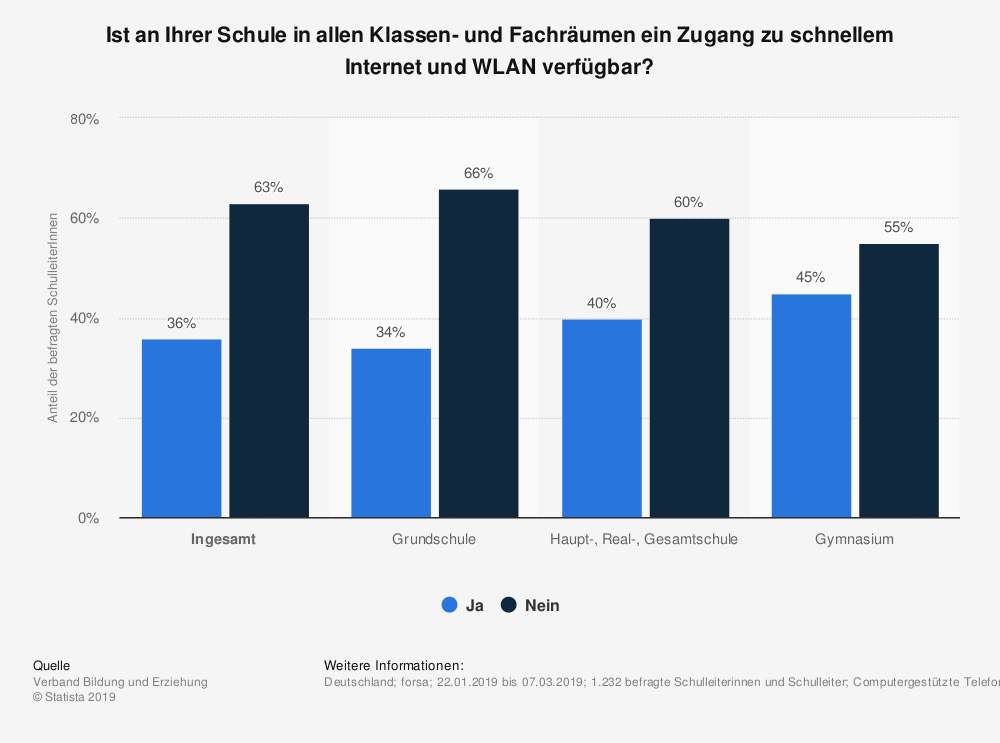
\includegraphics[width=0.9\linewidth]{bilder/statista_wlan}
	\caption[Verfügbarkeit von schnellem Internet und WLAN in Klassenräumen]{Verfügbarkeit von schnellem Internet und WLAN in Klassenräumen: Bundesweiten Erhebung zum Thema Digitalisierung an allgemeinbildenden Schulen in Deutschland. \cite{VBE2019}}
	\label{fig:statistawlan}
\end{figure}


Allerdings scheinen die ersten Barrieren durch den, in der  \hyperref[sec:einleitung]{Einleitung} dieser Arbeit bereits erwähnten, Digitalpakt Schule zu fallen. Dieser sieht vor fünf Millarden Euro in die IT-Ausstattung der deutschen Schulen fliesen zu lassen. Eine Schule mit mehr als tausend Schülern und entsprechendem Lehrkörper steht der Anforderungskomplexität an IT-Systeme eines größeren Wirtschaftsunternehmen kaum nach. Eine Ausnahme bilden hier Schulen, die auf professionelle Betreuung durch ein Systemhaus oder eigene Netzwerktechniker setzen \cite{Koenzen2018}. \\ \\ Eine interessante Alternative könnte hier das Nutzen von Cloud-Technologie sein. Cloud-basierte Netzwerkmanagementlösungen und Software-defined Networking (SDN) ist im Wirtschaftssektor bereits auf dem Vormarsch zu sein. Diese Technologien könnte Schulen dabei unterstützen den Digitalisierungsfortschritt voranzutreiben. Hierbei werden notwendige infrastrukturelle Geräte wie Access Points, Router, Switches und die nötige Verkabelung direkt vor Ort in der Schule installiert. Die Betreuung und Wartung erfolgt jedoch höchstmöglich automatisiert mit geringerem Aufwand aus der Ferne. 



\subsubsection{Ausblick digital gestützte interaktive Unterrichtsmethoden}\label{sec:interaktiveunterr}
Die erwähnte Technik im Abschnitt \ref{sec:digianschulen} macht den Einsatz von digital gestützten Interaktiven Unterrichtsmethoden möglich. Der online Lernvideo Anbieter Sofatutor hat im Jahr 2016 auf dem Educamp Leipzig Lehrerinnen und Lehrer über Software befragt, welche diese erfolgreich in ihren Unterricht integriert haben \cite{Sofatutor2019}. Neben zahlreicher Software, welche der Unterrichtsvorbereitung dient, lässt sich eine umfangreiche Liste in der Sektion "`Interaktion"' finden. Es lassen sich verschiedene Aufgabenformen ausmachen, die an einer digitalen Tafel von den Schülern gelöst werden sollen. Dies umfasst z.B. das Markieren, Sortieren, Zuordnen (Paare finden) von Bildern, Multiple-Choice Aufgaben, Brainstorming, Quiz-Anwendungen, u.v.m. Generell lässt sich feststellen, dass die Palette von Anwendungsmöglichkeiten enorm ist. Viele klassische Konzepte, die sich bereits analog interaktiv durchführen lassen konnten, stehen auch in einem digitalem Pendant bereit. Beispielsweise lassen sich Unterrichtsmethoden wie ein Lern-Quiz auch mit Papier und Stift durchführen, digitale Technik kann hier jedoch viel Arbeit abnehmen und lässt die Ausführung der Unterrichtsmethode deutlich immersiver und medial interaktiver zu. Abseits spielerischer Szenarien, kann z.B. die Mathematik Software \emph{GeoGebra} das Visualisieren von mathematischen Zusammenhängen. So Auswirkungen von anderen Werten gezeigt werden. Das Konzept "`bring-your-own-device"', welches vorsieht, dass Teilnehmende eigene Geräte mitbringen, wie z.B. ein Smartphone, steigert das Maß von Interaktivität zusätzlich. So ist es möglich, dass eine ganze Lerngruppe oder Schulklasse  an einer interaktiven Unterrichtsmethode simultan teilnimmt. Ebenso können Dozierende in einer Prüfungssituation auf Software zurückgreifen, welche die Prüfung der Teilnehmenden unterstützt und eine anschließende Auswertung der Antworten wesentlich automatisiert. An vielen Universitäten wird die Software \emph{Moodle} für diesen Zweck eingesetzt.  Zusammenfassend lässt sich feststellen, dass das Potential von digital gestützten Unterrichtsmethoden deutlich gegeben und das Angebot sowie das Potenzial der Anwendung vielfältig ist. Eine bewusste Einbettung in den Unterricht kann Dozierende unterstützen und entlasten. Als positiven Nebeneffekt lässt sich das Steigern von digitalen Kompetenzen seitens der Schülern vermerken, welche im Zuge der immer fortschreitenden weltweiten Digitalisierung eine nicht zu unterschätzende Fähigkeit ist. 
\newpage
\subsubsection{Datenschutz an Schulen}\label{sec:datenschutz}
Seit dem 25. Mai 2018 gilt die neue EU-Datenschutzverordnung, welche für alle Personen, Behörden oder sonstigen Stellen anzuwenden ist, wenn personenbezogene Daten verarbeitet werden. Dies betrifft also auch Schulen und ist sofern nichts neues, da die Datenverarbeitung und Auskunftsrechte in §64 des SchulG (Schulgesetz) im Falle des Bundeslands Berlin geregelt ist und dieser weiterhin anzuwenden ist. Neu ist allerdings, dass die Verantwortlichen für die Verarbeitung von personenbezogenen Daten weitere Aspekte berücksichtigen müssen, welche die neue Datenschutzverordnung mit sich bringt. Weiterführend sei hierzu die Quelle \cite[Datenschutz in der Schule]{Kachelriess2019} zu nennen. In diesem Zusammenhang ist es wichtig, dass auch eingesetzte Software an Schulen zu diesen Bestimmungen kompatibel sein muss, wenn diese personenbezogene Daten verarbeitet. Im Jahr 2018 an der Düsseldorfer Gemeinschaftsschule haben Unklarheiten um den Schutz von Schülerdaten dafür gesorgt, dass die Zeugnisse der rund 300 Schülerinnen und Schüler wieder per Hand geschrieben wurden. Auch die im vorherigen Abschnitt genannten Bring-your-own-device Praxis befindet sich Stand 2018 noch in einer rechtlichen Grauzone, sollten personenbezogene Daten verarbeitet werden\cite{WitmerGossner2018}. Die im Abschnitt \ref{sec:technikunterricht} genannte Auslagerung in eine Cloud könnte hier ebenfalls helfen, wenn der Cloud-Anbieter EU-Datenschutzverordnung konform arbeitet. Zur Einhaltung der gesamten Datensicherheit, ist es auf jeden Fall ratsam, wenn Cloud-Anbieter und Server ihren Standort in Deutschland haben.
Verlassen Daten alternativ gar nicht erst das Schulgelände, trägt dies ebenso positiv zum Erhalt des Datenschutzes bei.  
\newpage


\subsection{Überblick Webtechnologie}\label{sec:webbasedsoftware}
% Hier auf PDF Technische Anforderungen verweisen (Footnote?) da sehr ausführlich und gut
% Anfang Geschichtlich
In den folgenden Untersektionen \ref{sec:websoftpopular} ff. wird ein Überblick über Webtechnologie und Web-Softwareentwicklung gegeben.

\subsubsection{Popularität}\label{sec:websoftpopular}
Seit dem Erfolgskurs des Web 2.0\footnote{Web 2.0 ist ein Schlagwort, das für eine Reihe interaktiver und kollaborativer Elemente des Internets, speziell des World Wide Webs, verwendet wird. Dabei konsumiert der Nutzer nicht nur den Inhalt, er stellt als Prosument selbst Inhalte zur Verfügung. - Wikipedia.org} in den frühen 2000er Jahren, zeichnet sich zunehmend der Trend des Software-as-a-Service Geschäftsmodells ab. Dies beschreibt die Bereitstellung von Software im Internet oder durch ein lokal laufenden Servers, ohne dass Benutzende die Software selbst noch lokal installiert haben müssen. Im Jahr 2015 setzten bereits über drei Viertel von 102 befragten Unternehmen Software dieser Form aktiv im Geschäft ein \cite{TecArt-GmbH2019:online}. Viele Arten von Software können  mittlerweile in einer im Webbrowser lauffähigen Alternative substituiert werden. Ein populäres Beispiel ist die Office-Suite \emph{Google Docs} der Firma \emph{Google inc.} Hier lassen sich Textverarbeitung, Tabellenkalkulation und das erstellen von Präsentationen ohne Installation und direkt im Webbrowser des Benutzenden ausführen. Ein anderes Beispiel ist die Web-Software \emph{Photopea} welche ebenfalls komplett im Web-Browser ausgeführt wird und dem nur lokal installiert ausführbaren Bildbearbeitungsprogramm \emph{Photoshop} der Firma \emph{Adobe inc.} sehr nahe kommt. Im Vergleich zu lokal installierter Software ist die Bereitstellung von Web-Software einfacher, da solange ein moderner Webbrowser lauffähig ist, das Betriebssystem des Client-Computers zu vernachlässigen ist. Ebenso stellt potente Hardware keine zwingende Voraussetzungen, da etwaige rechenintensive Aufgaben auf der Serverseite getätigt werden können oder hier eine Balance zwischen Client und Server angestrebt werden kann. \\ 

\subsubsection{Intranet und Internet}\label{sec:intranetundinternet}
% Detailgrad so sinnvoll?
% Unterschied und Gemeinsamkeit klar machen
% Hier kommunikation erklären! Protokolle und OSI schicht!
Einfach ausgedrückt, ist das Internet ein Netzwerk von Computern, welche weltweit miteinander vernetzt sind. Seine Anfänge lassen sich auf das Ende der 1960er in den USA datieren, als die DARPA (Defense Advanced Research Projects Agency) eine weltweite Verknüpfung von Datennetzen anstrebte. Das hier draus resultierende ARPANET (Advanced Research Projects) kann als Ursprung angesehen werden. Dabei beschreibt der Begriff Internet streng genommen ein 'interconnected network', also ein international vernetztes Netzwerk, ohne dabei die Hardware- und Netzwerktechnologie genauer zu beschreiben \cite{Safran2011}.  \\ 
Die wohl populärste Anwendung des Internets ist das World Wide Web, welche gegen das Jahr 1989 von einer Forschungsgruppe rund um Sir Tim Berners-Lee ins Leben gerufen wurde und heute oftmals als Synonym für das gesamte Internet sprachlich genutzt wird. \\ 

In unser heutigen globalisierten Welt lässt sich das Internet mitsamt World Wide Web nicht mehr wegdenken und ist ein integraler Bestandteil der Kultur und Struktur des weltweiten Informationsaustausches.
 \\ \\
 Das Intranet beschreibt analog dazu ein lokal abgeschlossenes Netzwerk von Computern, bspw. innerhalb eines Unternehmens. Dabei endet ein Intranet an seinen Grenzen und ein Gateway fungiert als Übergabepunkt ins Internet (siehe Abbildung \ref{fig:intranetinternet}). Die Vernetzung der Endgeräte erfolgt kabelgebunden (LAN) oder kabellos (WLAN). Die Kommunikationsgeschwindigkeit innerhalb eines Intranets sind i.d.R. deutlich höher als im Internet, da Daten nicht erst nach außen an einen Internet Service Provider übermittelt werden müssen. Ein Intranet funktioniert unabhängig vom öffentlichem Internet (erhöhte Ausfallsicherheit), ist nicht öffentlich zugänglich und bietet oft andere oder zusätzliche Funktionen \cite{Intranet62:online}. 
 
 \begin{figure}[H]
 	\centering
 	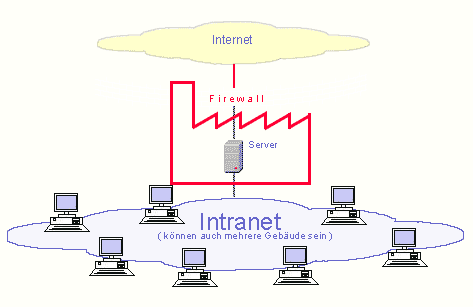
\includegraphics[width=0.8\linewidth]{bilder/intranetinternet}
 	\caption[Schematische Darstellung Intranet und Internet]{Schematische Darstellung Intranet und Internet \cite{intranet2019}}
 	\label{fig:intranetinternet}
 \end{figure}
 

 \subsubsection{Client-Server Modell}\label{sec:clientservermodell}
 Das Client-Server Modell beschreibt das Prinzip der Kommunikation zwischen zwei Teilnehmern innerhalb eines Netzwerks. Grundlegend unterscheidet das Modell hierbei zwischen einer Anbieterseite (Server) und einer Benutzerseite (Client). Der Client betreibt auf seinem Endgerät (Computer, Smartphone, etc.) eine Client-Software mit der die Verbindung zum Server aufgebaut wird. Im Fall des WWW (siehe \ref{sec:www}) ist dies in den meisten Anwendungsszenarien ein Webbrowser. Der Client fordert dabei eine Ressource an, welche auf dem Server vorliegt oder dort speziell für die Anfrage des Clients generiert wird (siehe auch Sektion \ref{sec:webanwenservices}). Das Client-Server Modell sieht vor, dass immer der Client die Verbindung aufbaut, nie andersherum \cite{ElektronikKompendium.de:online}. Die Anfrage des Clients wird \emph{Request} genannt, die Antwort des Servers \emph{Response} oder \emph{Reply}, welche bei ausreichender Berechtigung des Clients auch Daten enthält. 
 Server-Computer sollen rund um die Uhr erreichbar sein, während Client-Endgeräte auch abgeschaltet werden können, ohne die Integrität des Netzwerks zu beeinflussen. 
  % Vergleich zu anderen Modellen?
 
\subsubsection{Kommunikation}\label{sec:kommunikation}
Die Kommunikation im Internet und Intranet erfolgt über Protokolle. 
Ein Protokoll kann als ein Satz von Kommunikationsregelvorschriften \cite{Safran2011} verstanden werden, welche den Netzwerkverkehr auf unterschiedlichen Schichten reglementieren. 
Diese Schichten werden im \emph{OSI-Modell} (Open System Interconnection) der \emph{ISO} (International Standardization Organisation), der internationalen Standardisierungsorganisation beschrieben. 
\\ 
Das \emph{ISO-OSI-Modell} ist dabei in sieben Schichten eingeteilt, während die Erste als physikalische Schicht definiert ist und die Siebte als Anwendungsschicht. Protokolle sind dabei jeweils nur über Protokolle benachbarter Schichten in Kenntnis gesetzt. Es lässt sich grob in anwendungsorientierte Schichten (1 bis 4) und transportorientierte Schichten (5 bis 7) unterteilen. Die im Rahmen dieser Arbeit genutzten Webtechnologien nutzen kommunikativ nur anwendungsorientierte Schichten des \emph{ISO-OSI Modells}.



% Begriff Internet
\subsubsection{World Wide Web}\label{sec:www}
Das \emph{World Wide Web} (WWW) ist die wohl populärste Anwendung des Internets~\cite{Safran2011} und wird oftmals fälschlicherweise als Synonym für das gesamte Internet genannt. Das WWW ist eine Sammlung von verteilten Dokumenten, welche sich gegenseitig über sog. Hyperlinks referenzieren und von Web-Servern zur Verfügung gestellt werden. Auf der Client Seite (siehe \ref{sec:clientservermodell}) stellt der Web-Browser die wichtigste Software da. Mit ihr werden Web Server angesprochen (Request) und Antworten (Response) für den Nutzenden dargestellt. Die wichtigsten sprachlichen Komponenten des WWW sind: \\ 
\begin{itemize}
	\item \textbf{HTML:} Hypertext Markup Language - eine reine Beschreibungssprache, welche Hypertext Dokumente durch Tags codiert. 
	\item \textbf{CSS:} Cascading Style Sheet - Eine Stylesheet-Sprache, welche das äußere Erscheinungsbild von Hypertext Dokumenten beschreibt
	\item \textbf{JS:} JavaScript: Eine Skriptsprache, welche u.A. Interaktion sowie Dynamik hinzufügt und clientseitig interpretiert wird. 
\end{itemize}
Die Techniken des WWW können auch lokal im Intranet genutzt werden. 
Das zur Verständigung zwischen Client und Server genutzte Protokoll (siehe \ref{sec:kommunikation}) ist das \emph{Hypertext~Transfer~Protocol} (HTTP) bzw. in verschlüsselter Form \emph{Hypertext~Transfer~Protocol~Secure} (HTTPS), da eine Übermittlung im Klartext nicht immer wünschenswert ist. HTTP/HTTPS ist ein Zustandsloses Protokoll, das bedeutet dass jede Anfrage unabhängig voneinander geschieht und betrachtet wird. Dies und die Tatsache, dass jede Anfrage von der Client-Seite aus gestartet werden muss (siehe \ref{sec:clientservermodell}), stellen oftmals Hürden für die Entwicklung von Webanwendungen und Webservices da. Techniken wie \emph{Cookies} und \emph{Sessions}, sowie das wiederholte Abfragen von aktualisierten Daten seitens des Clients wirken hier entgegen. \emph{Cookies} stellen persistent gespeicherte Daten auf der Client-Seite da, mit deren Hilfe der Webserver einen Client eindeutig zuordnen kann. Bei einer \emph{Session} sendet der Client bei jeder Anfrage eine eindeutige ID an den Server. Im Normalfall endet eine Session beim Beenden des Webbrowser, während Cookie-Dateien eine längere Lebensdauer besitzen.      
%
\subsubsection{Webanwendungen und Webservices}\label{sec:webanwenservices}
Im Laufe der Entwicklung des WWW (siehe \ref{sec:www}) stieg der Anspruch vom reinen Anbieten statischer Dokumenten in Richtung dynamischer Inhalte, welche einer Programmlogik folgend von einem Webserver für jede Anfrage generiert werden. Web\-anwendungen sind Computerprogramme, welche auf einem Webserver ausgeführt werden und den Webbrowser des Clients als Schnittstelle nutzen \cite{Safran2011}. Dies bietet den großen Vorteil, dass etwaige Anpassungen von Programmlogik nur serverseitig erfolgen müssen und jeder Client mit Webbrowser als Benutzerschnittstelle ausreicht. \\ \\
Webservices sind eine spezialisierte Art von Webanwendung. Der Fokus hier liegt auf dem Bereitstellen von Daten für andere Applikationen, welche die gewonnen Daten selbst auswerten und dem Nutzenden bereitstellen. Dies geschieht i.d.R. über eine einheitlich beschriebene Schnittstelle (API - \emph{Application Programming Interface}), über welche fremde Applikationen angefragte Daten abrufen können. Der Austausch der Daten erfolgt hier meist über Formate wie JSON (\emph{JavaScript Object Notation}) oder XML (\emph{Extensible Markup Language}), da Aussehen und Lesbarkeit der Daten irrelevant sind und somit eine Ausgabe in HTML nicht von Nöten ist. \\
Bei der Implementierung eines Webservices bieten sich folgende zwei technologische Arten der Umsetzung an: \\ \\
\textbf{SOAP/WSDL}: Hier werden Nachrichten über das \emph{Simple Object Access Protocol} (SOAP) ausgetauscht und deren Beschreibung über die \emph{Web Services Description Language} (WSDL) definiert. Anfrage- und Antwortformat der Daten ist XML, eine Auszeichnungssprache, welche HTML sehr ähnelt aber deutlich allgemeiner ist. XML kann also mehr als Regelwerk verstanden werden, mit dessen Hilfe Entwickelnde ihre eigene hierarchische Beschreibung einer Datenstruktur vornehmen können. XML und HTML leiten sich bei der von der SGML (\emph{Standard Generalized Markup Language}) ab, welches ihre Ähnlichkeit zusätzlich begründet \cite{XMLHTMLU88:online}. \\

 
\textbf{REST}: Representational State Tranfer - Hier kann jede einzelne Funktion des Webservices über eine jeweils zugeordnete URL (\emph{Uniform Resource Locator}) abgerufen werden, umgangssprachlich als Webadresse bekannt. Das WWW selbst kann als REST-Webservice verstanden werden \cite{Bayer2002:online}. \\ 

\subsection{Websockets}\label{sec:websockets}
Bezugnehmend auf die Problematik, welche durch die Kommunikationsstrategie über das http-Protokoll entsteht (siehe Sektion \ref{sec:www}), wirken \emph{Websockets} dieser entgegen. Als Kommunikationskanal verknüpft ein \emph{Websocket} Server und Client. Zwar muss die Kommunikation zunächst über den Client initiiert werden, bleibt dann jedoch bestehen und der Server kann diese nutzen um aktiv neue Daten zu emittieren. Ein Nachteil ist jedoch, dass im Gegensatz zum http-Protokoll hier auch Daten hin- und hergeschickt werden, wenn dies eventuell nicht gewünscht ist~\cite{neumann2015entwicklung}, was insbesondere bei mobilen Applikationen kritisch sein kann. Ein generellen Vorteil bieten \emph{Websockets} auch in Sachen Performanz, da das Protokoll, ist erst einmal eine Verbindung zustande gekommen, deutlich schlanker ist. \\ Die folgende Abbildung \ref{fig:socketsrest} zeigt einen Performanz Vergleich in Anbetracht des zusätzlichen \emph{Payloads} von REST- und \emph{WebSocket} Nachrichten. 

\begin{figure}[H]
	\centering
	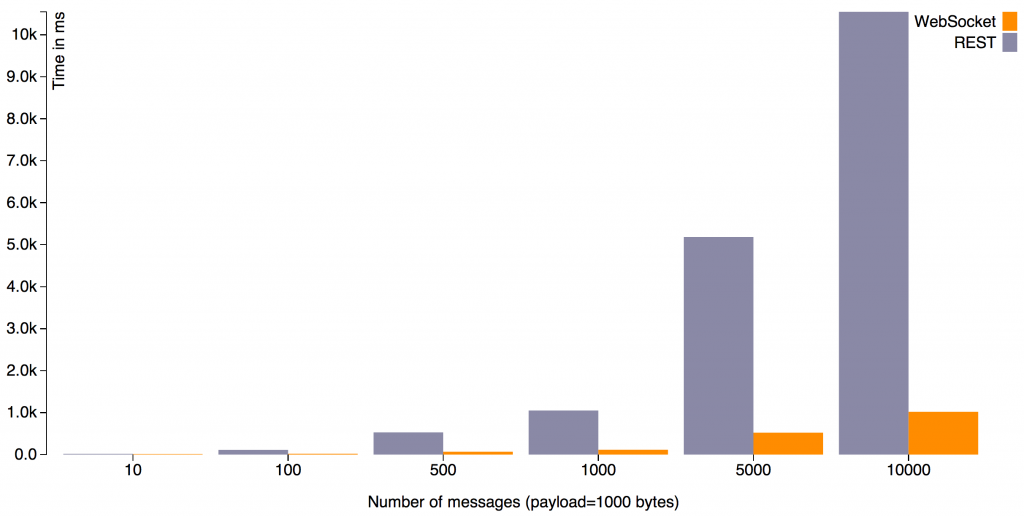
\includegraphics[width=0.9\linewidth]{bilder/websocket-rest-messages}
	\caption[Performanzvergleich REST versus WebSockets]{Performanzvergleich REST versus WebSockets \cite{Gupta2014}: \\ Benötigte Zeit um N Nachrichten einer konstanten Nachrichtengröße zu verarbeiten.}
	\label{fig:socketsrest}
\end{figure}

\subsection{Webapplikationsentwicklung}\label{sec:softwareentwicklung}
Dieses Kapitel beleuchtet wesentliche Begriffe hinsichtlich der Entwicklung von Webapplikationen.
Webanwendungen und Webservices können unter diesem Begriff zusammengefasst werden.
\\ 
\subsubsection{Web-Application-Frameworks} \label{sec:wafs}
Bei der Entwicklung von Webapplikationen wird oftmals auf Frameworks, spezifischer Web-Application-Frameworks (WAF) zurückgegriffen. 
Ein WAF bezeichnet ein Programmgrundgerüst, welches als Grundlage im Implementierungsprozess zum Einsatz kommt \cite{Ionis2019:online}. Dies erleichtert die Entwicklung ungemein, da auf bereits vorgefertigte Ansätze und Programmbausteine zurückgegriffen werden kann. Diese WAFs reflektieren zumeist auch Modelle und Prinzipien, was einen gewissen Grad an Konformität gewährleistet und das Verständnis für den Quellcode erhöht.
Ein für Frameworks bekanntes Paradigma stellt das Umsetzungsparadigma \\
\textbf{Inversion of Control} (IoC), z. Dt. Umkehrung der Steuerung dar, welches u.a. auch in der objektorientierten Programmierung Anwendung findet.
Hierbei wird eine Funktion/Unterprogramm bei der Hauptprogrammbibliothek registriert und von dieser zu einem späteren Zeitpunkt aufgerufen. Dies ist umgangssprachlich auch als 'Hollywood'-Prinzip bekannt ("`Don't call us! We call you"' z. Dt. "`Ruf nicht uns an! Wir rufen dich an!"'). Das Framework behält also die Programmflusssteuerung bei. 
  Ein Nachteil, der durch den Einsatz von eines WAFs bedingt ist, stellt die Einschränkung der Freiheit während des Implementierungsprozesses dar. Dieser wird jedoch billigend in Kauf genommen, da sich ein Reduktion des Zeit- und Kostenaufwands erhofft wird. Die Wahl des richtigen WAFs ist ein wichtiger Entschcheidungsprozess, bei dem mehrere Faktoren beachtet werden müssen, wie z.B. benötigte Einarbeitungszeit und Lizenzen.

\subsubsection{Serverseitiger Ansatz}\label{sec:serverseitgeransatz}
Anknüpfend an Sektion \ref{sec:webanwenservices} sind Webapplikationen Software, welche serverseitig ausgeführt werden, wobei der Webbrowser eines Nutzenden als Benutzerschnittstelle dient. Eine Webapplikation kann jedoch auch clientseitig implementiert werden, wie in Sektion \ref{sec:clientseitigeransatz} beschrieben. \\ 
Serverseitige Webapplikationen verfolgen oftmals den \emph{Multi-Page} Ansatz, das heißt pro Anfrage (Request) wird dem Client (Webbrowser) ein anderes Dokument  übergeben. Wichtige Programmiersprachen für den Ansatz sind \emph{php}, \emph{Ruby}, \emph{Python}, \emph{Java} und auch \emph{JavaScript}. Letzteres kam zuvor nur auf der Clientseite zur Anwendung. \\
Die \textbf{Model - View - Controller} Architektur (MVC) ist die vorherrschende Architektur, auf welche sich der Großteil der serverseitigen WAFs stützen.
Hierbei wird die Programmlogik klar in drei große Bestandteile unterteilt: \\ \\
\textbf{Model}: Das Model oder z. Dt. Modell (im restlichen Teil der Ausarbeitung \emph{Model} geschrieben) beschreibt eine Datenstruktur an sich. In einem Webshop wären dies z.B. die Produkte und deren Eigenschaften wie ID, Name, Preis usw. \\
\textbf{View}: Sie beschreibt die reine Ansicht eines \emph{Models}. In einem Webshop wäre dies z.B. die Detailseite eines Produkts. \\
\textbf{Controller}: Der Controller dient als Bindeglied zwischen \emph{Model} und \emph{View}. Er handelt ankommende \emph{Requests} (Anfragen) ab und übergibt der \emph{View} aus dem Modell die notwendigen Daten. \\ 
Neben der MVC Architektur existieren weitere, andere Architekturen und Ableitungen der MVC Architektur, wie z.B. der im \emph{Django} WAF genutzten \emph{Model - View - Presenter} Architektur. \\
Die folgende Tabelle \ref{tab:servwaf} zeigt einen groben Überblick über bekannte WAFs, welche den serverseitigen Multi-Page Ansatz verfolgen \cite{TopWebDe0:online}. 

\begin{table}[H]
	\centering
	\caption{Überblick einiger serverseitiger Web-Application-Frameworks}
	\label{tab:servwaf}
	\begin{tabularx}{0.8\textwidth}{llX}
		\textbf{Name} & \textbf{Sprache} & \textbf{Architektur}   \\ 
		\toprule
		Symfony & php & Model - View - Controller \\
		\rowcolor[HTML]{EFEFEF} 
		Laravel	& php & Model - View - Controller  \\ 
		Phalcon	& php & Model - View - Controller   \\
		\rowcolor[HTML]{EFEFEF}  
		Codeigniter & php & Model - View - Controller \\
		Django & Python & Model - View - Presenter \\	
		\rowcolor[HTML]{EFEFEF} 	
		Ruby on Rails & Ruby & Model - View - Controller \\
		\hline 
	\end{tabularx} 
\end{table}


Aus der Tabelle lässt sich eine starke Popularität der Programmiersprache \emph{php} ableiten und deren auf dieser Sprache basierenden WAFs. Die Tabelle stellt keinen Anspruch auf Vollständigkeit, da noch unzählig viele andere serverseitige WAFs existieren. Ebenso wurde das WAF \emph{ExpressJS}, welches auf der serverseitigen Plattform \emph{NodeJS} basiert, bewusst nicht mit in die Tabelle aufgenommen, da dies ein Sonderfall darstellt. Diese Thematik wird in Kapitel \ref{sec:konzept} ausführlich behandelt. 
%Hier über NodeJS und PHP quatschen!
\subsubsection{Clientseitiger Ansatz}\label{sec:clientseitigeransatz}
 Das Programmiermodell des WWW, welches durch die Architektur des HTTP geprägt ist, wird bei der Entwicklung von Webapplikationen übernommen. Dies sieht eine Anfrage immer seitens des Clients vor (siehe auch Sektion \ref{sec:www}). Dies schränkt das Ausmaß von Interaktion und generieren von dynamisch ladenden Webseiten ein. 
 Der clientseitige Ansatz der Webapplikationsentwicklung kommt meistens bei sog. Single-Page-Applikationen zur Anwendung. Hierbei wird o.g. Problem damit umgangen, indem bei Aufruf einer Internetseite die gesamte HTML Benutzeroberfläche inklusive Programmlogik in Form von JS Code als Ganzes an die Client übergeben wird. Dies bietet den großen Vorteil, dass die Logik nun auf dem Client ausgeführt wird und dieser dynamisch Daten nachladen bzw. Anfragen kann. Oftmals ändert sich auf einer Single-Page Applikation die Webadresse in der Adresszeile des Browsers nicht. Die ganze Applikation läuft also auf einer einzelnen Website ab, die sich dynamisch ändert. Dieses dynamische Nachladen von Inhalten wird \textbf{AJAX} - \emph{Asynchronous JavaScript and XML} genannt.  Die einzig nativ unterstützte Programmiersprache seitens der Webbrowser ist \emph{JavaScript} und daher vorherrschend \cite{Safran2011}.
 Jeder moderne Webbrowser hat einen JS Interpreter integriert. Über Plugins können zwar auch andere Sprachen genutzt werden, in Form von \emph{Java-Applets} (Programmiersprache dort \emph{Java}) oder das früher sehr populäre \emph{Flash} des Unternehmens \emph{Adobe}, welches \emph{ActionScript} als Programmiersprache nutzt. Beides gilt aber Stand 2019 als veraltet und der Einsatz derartigen Technologien wird nicht empfohlen. %Nachweis nötig?
Es gibt sehr viele JavaScript WAFs und Bibliotheken, zu den bekanntesten zählen: \\ \\ 
% hier noch bisschen mehr vielleicht
 \textbf{Angular} ist ein clientseitiges \emph{JavaScript} WAF, entwickelt und bereitgestellt von dem Unternehmen \emph{Google inc}. Es hat vergleichsweise eine steile Lernkurve und setzt etwas Einarbeitungszeit voraus. \\ \\
 \textbf{React} ist streng genommen kein WAF, sondern lediglich eine JS Bibliothek. Es bietet aber über Erweiterungen die Möglichkeit, wie ein WAF genutzt werden zu können, was seine Flexibilität noch erhöht. Entwickelt und Betrieben wird \emph{React} von der Firma \emph{Facebook inc.} \\ \\
 \textbf{Vue} ist ein clientseitiges \emph{JavaScript} WAF, ursprünglich entwickelt von dem Entwickler Evan You. Es gilt als einfacher zu erlernen als \emph{Angular} und ist sehr flexibel. \\ 
 
 
 Das Entwickeln von clientzentrischen JS Anwendungen ist mittlerweile so fortgeschritten, dass oftmals beim Nutzenden ein Gefühl entsteht, es würde ein lokal installiertes Programm ausgeführt werden. Populäre Beispiele wäre das in Kapitel \ref{sec:zielsetzung} erwähnte \emph{Google Docs}, welches eine voll umfassende Textverarbeitungslösung im Browser bietet. Derartige Applikationen werden \emph{Rich Internet Application} (RIA) genannt.
 

%Hier vor allem über Javascript quatschen!
\subsubsection{Hardware Anforderungen}\label{sec:hardware}
Auf der \textbf{Serverseite} ist der Anspruch an die Hardware sehr abhängig vom gewünschten Anwendungsfall und benötigter Skalierbarkeit. Das beliebte Server \emph{Linux} Derivat \emph{Debian} benötigt bspw. mindestens 128~Megabyte Ram-Speicher und 2~Gigabyte Festplattenspeicher. Es ist aber durchaus möglich mit noch sehr viel weniger potenter Hardware ein Server zu betreiben \cite{dpakt2019:online}. 
Für den Einsatz in einzelnen Unterrichtsklassen an Schulen würde ein \emph{Raspberry Pi 3} Einplantinencomputer bereits genügend Leistung für Webanwendungen und einen günstigen Anschaffungspreis bieten. Auch besitzen bereits 67\% der 10 bis 11 jährigen Jugendlichen Smartphones \cite{Statista2017:online}, welche ebenfalls genug Leistung für Webanwendungen aufweisen und als Clients genutzt werden können. \\ 
\subsubsection{Vergleich zu anderen Entwicklungsansätzen}\label{sec:vorundnachteileweb}
Der klassische Ansatz der Software Entwicklung wäre das Implementieren eine Desktop-Anwendung, welche lokal
auf dem Computer des Anwendenden installiert wird. Typischerweise wird die Software programmiert und anschließend von einem Compiler in Maschinencode übersetzt bzw. von einer Laufzeitumgebung zur Ausführung interpretiert. Die Software wird also normalerweise auf dem Computer installiert und an die Gegebenheiten des Betriebssystems angepasst. Dies hat den Vorteil bei Bedarf sehr hardwarenah und performant entwickeln zu können, was durch das vorherige kompilieren des Codes in Maschinencode begünstigt wird. Nachteilig ist es jedoch, dass die Software zunächst überhaupt installiert werden muss. Eine noch vergleichsweise neue aber vielversprechende Webtechnologie ist in dieser Hinsicht \emph{Webassembly} (WASM). Dies ist ein Bytecode, welcher neben der virtuellen JS-Maschine im Webbrowser ausgeführt wird und aus Programmiersprachen wie \emph{C}, \emph{C++} oder \emph{Rust} kompiliert wird. Dies soll die Monopolstellung von JS als einzig ausführbare Sprache im Webbrowser adressieren und vor allem auf rechenintensiven Anwendungsgebieten einen Vorteil erbringen \cite{Stueckler2018}. \\  Die folgende Tabelle \ref{tab:vergleichwebdesk} vergleicht Web- und Desktopapplikationen hinsichtlich gängiger Kriterien.

\begin{table}[H]
	\centering
	{\footnotesize
	\caption{Vergleich von Web- und Desktopapplikationen \cite{TecArt-GmbH2019:online}}
	\label{tab:vergleichwebdesk}
	\begin{tabularx}{\linewidth}{l  X  X}
		\textbf{Kriterium} & \textbf{Webapplikation} & \textbf{Desktopapplikation}   \\ 
		\toprule 
		Struktur & Modularer Aufbau & Meist als Gesamtpaket vertrieben \\
		\rowcolor[HTML]{EFEFEF} 
		Verfügbarkeit & Weltweit dank Internet, \newline lokal eingeschränkt möglich & Nur bei lokaler Installation verfügbar \\ 
		
		Installation	& Nicht erforderlich & Erforderlich   \\ 
		\rowcolor[HTML]{EFEFEF} 
		Speicher & Kein Zusätzlicher Speicher benötigt & Installation benötigt Speicherplatz \\
		
		Updates & Live-Aktualisierung möglich & Teil- oder Neuinstallation notwendig \\		
		\rowcolor[HTML]{EFEFEF} 
		Teamarbeit & Zeitgleiches und schnelleres Arbeiten leicht möglich & Teamarbeit nur über Synchronisation möglich \\
		
	\end{tabularx}
	}
\end{table}


\newpage

\input{sections/04Analyse}
\newpage

\section{Konzept}\label{sec:konzept}
Dieses Kapitel stellt das Konzept zur Realisierung des Projekts vor. 
Dies umfasst den allgemeinen Systemaufbau, sowie Architekturentwürfe hinsichtlich der Server- und Clientseite inklusive den im Verbund eingesetzten Softwaremodulen.
\subsection{Systemaufbau}\label{sec:sysaufbau}
Das System soll in eine Server- und Clientseite aufgeteilt sein. 
Da es sich um eine Webapplikation handeln soll, wird die Interaktion mit dem Server über einen Webbrowser stattfinden und dieser soll auch gleichzeitig der Client sein. Für Aufgaben wie das Starten des Servers, soll die Steuerung über die Kommandozeile des Host-Computers möglich sein. Alle anderen Interaktionen werden über den Web-Clients ausgeführt.
\subsection{Netzwerkaufbau}\label{sec:netzwerkaufbau}
Als Kommunikationsprotokoll soll das aus dem Webbereich bekannte HTTP resp. HTTPS Protokoll zum Einsatz kommen. Der Server wird als Webserver fungieren, Anfragen müssen vom Client aus initiiert werden (vgl. Abschnitt \ref{sec:www}). Bei Parts, welche Echtzeitinteraktion benötigen, soll das Websocket (ws) Protokoll zum Einsatz kommen, welches eine bidirektionale Kommunikation zwischen Server und Client ermöglicht. Der Server soll sowohl in einem Intranet wie auch im Internet lauffähig sein. Dabei kann er, je nach infrastruktureller Realisierung über ein IPv4 oder IPv6 Adresse erreicht werden, bei Nutzung eines DNS-Servers auch über eine Domain.\\ \\

Der Kommunikationsaufbau ist schematisch in Abbildung \ref{fig:server_kommdiagram} dargestellt. 

\begin{figure}[H]
	\centering
	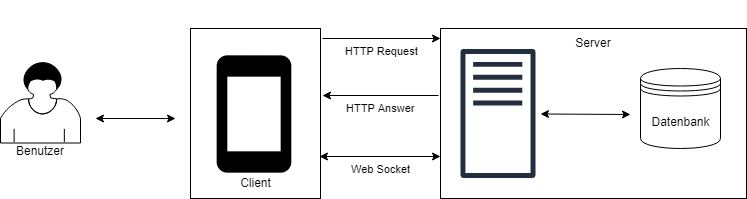
\includegraphics[width=0.8\linewidth]{bilder/server_diagram}
	\caption[Kommunikationsaufbau des zu entwickelnden Systems]{Kommunikationsaufbau des zu entwickelnden Systems}
	\label{fig:server_kommdiagram}
\end{figure}


\subsection{Entwurf des Servers}\label{sec:serverkonzept}
Aufbauend auf das Grundlagen- und Analysekapitel sollen in diesem Abschnitt die Lösungen hinsichtlich der Serverkomponente des Projekts aufgezeigt werden. 
\subsubsection{Laufzeitumgebung: Node.js}\label{sec:nodejs}
Als Laufzeitumgebung und Grundbaustein des Servers wird die JavaScript-""Laufzeitumgebung \emph{Node.js} \cite{Node.js} genutzt werden, da dies zwei wesentliche Vorteile mit sich bringt:
\begin{enumerate}
	\item \emph{Node.js} nutzt als Paketmanager und Projektverwaltungstool \emph{Node Paket Manager} (NPM). Mit dieser Software ist der Zugang zu über 350.000~Paketmodulen (Stand 13. Januar 2017) \cite{npm2017} gegeben und diese können das Projekt Modular erweitern. Diese können in \emph{Node.js} gemäß dem IoC Prinzips genutzt werden (siehe auch Abschnitt \ref{sec:wafs}). 
	Ebenso können mit NPM grundlegende Start- und Installationsskripte leicht ausgeführt werden. 
	\item Da \emph{Node.js} eine JavaScript-Laufzeitumgebung ist, wird zur Programmierung die Skriptsprache \emph{JavaScript} genutzt, welche auch auf der Clientseite im Webbrowser zum Einsatz kommt. Dies erleichtert den Implementierungsprozess, da einheitlich in einer Sprache geschrieben wird.
\end{enumerate}
Darüber hinaus können NPM-Pakete auch auf der Clientseite genutzt werden (siehe dazu auch Abschnitt \ref{sec:browserify}). Eine gute Skalierbarkeit ist ebenfalls gegeben. Dies wird in folgenden Abschnitten genauer erläutert. Ist ein besonders hoher Ressourcenbedarf von Nöten (z.B. eine Bildungseinrichtung möchte einen zentralen Server installieren, welche viele Klassen/Kurse bedienen soll) können mehrere Serverinstanzen auf einem Computer parallel laufen und vorab mit einem Lastenverteiler (Load Balancer) Server, wie z.B. \emph{NGINX} verwaltet werden. Um dies zu erreichen wird das Projekt mit \emph{Node.js} realisiert werden und nicht mit einem \emph{php}-Framework. \\ Da \emph{Node.js} grundlegend sehr offen ist was seinen Einsatzzweck betrifft, soll als Webserver Modul das NPM-Modul \emph{Express} genutzt werden, welches im nächsten Abschnitt genauer erläutert wird.
\subsubsection{Webserver: Express}\label{sec:expressjs}
Um mit Node.js komfortabel eine Webapplikation zu implementieren, soll das bekannte Webserver-Framework \emph{Express} eingesetzt werden, welches viele HTTP-""Dienstprogrammmethoden und den Einsatz von Middlerwarefunktionen gestattet. Hierbei wird jeder eingehende HTTP Anfrage von Funktion zu Funktion weitergeleitet (Aufruf der Methode \texttt{next()}) oder explizit beantwortet (die Funktion besitzt ein Rückgabewert). Ebenso ist mit \emph{Express} das Abbilden von Routen möglich. \emph{Express} wird für den gesamten administrativen Teil des Lehrer-Login zum Einsatz kommen. Ebenso soll durch \emph{Express} das Anlegen und Editieren von Lehreinheiten möglich sein (vgl. Sektion \ref{sec:sysbeschreib}). 
Da für den gesamten Lehrer-Backendbereich \emph{Express} zum Einsatz kommen soll und hier mit einfachen HTTP-Requests gearbeitet wird, kann der Einsatz von JavaScript auf der Client-Seite auf ein Minimum reduziert werden, was dem Einsatz auf Servereinheiten mit nicht modernen Webbrowsern entgegenkommt (sollte Client und Server auf der gleichen Maschine ausgeführt werden).\\ \\ 
Für den interaktiven Part des Projekts werden zur Kommunikation \emph{WebSockets} genutzt, welche mithilfe der JavaScript-Bibliothek \emph{Socket.IO} realisiert werden sollen. Dies wird in der nächsten Sektion beschrieben.   

\subsubsection{Socket.IO}\label{sec:socketio}
Die JavaScript-Bibliothek \emph{Socket.IO} \cite{Socket.IO2019} ermöglicht bidirektionale Echtzeit-\\Kommunikation zwischen Webclient und Server, wobei jeweils ein Bibliotheksteil auf Server- und Clientseite zum Einsatz kommt. Ein großer Vorteil ist, dass beide Komponenten eine nahezu identische API aufweisen. Daten können sehr einfach von Client ereignisgetrieben (event-driven) zwischen Server und Client sowie vice versa ausgetauscht werden. Client und Server lauschen dabei gegenseitig auf Ereignisse, wie das Verbinden eines neuen Clients oder auch selbst implementierte Ereignisse. Dabei können jegliche \emph{JavaScript} Daten hin-und hergeschickt werden. Eine händische Konvertierung in das JSON-Format ist nicht notwendig. \emph{Express} wird zunächst Client Daten (HTML-, CSS- und JS- Daten) auf einer festgelegten Route senden. Anschließend wird die Kommunikation von \emph{Socket.IO} gesteuert. 
\subsubsection{Sonstige Module}
Neben \emph{Express} ist der Einsatz von weiteren Modulen (\emph{Node Packages}) vorgesehen, welche unterschiedliche Funktionen realisieren sollen. Diese sind:
\begin{itemize}
	\item \textbf{Body-Parser}: Diese Modul ermöglicht das einfach Auslesen von HTTP-Requests. Schickt ein Client bspw. Formulardaten, können diese einfach gelesen und ausgewertet werden. 
	\item \textbf{express-session}: Da Lehrende und Administratoren zur Nutzung der Software einen gültigen Zugang besitzen müssen, sind zur Authentifizierung der Nutzenden HTTP-Sessions vorgesehen (vgl.  Abschnitt\ref{sec:www}). Das Modul \emph{Express-Session} macht das Arbeiten mit diesen sehr komfortabel. Über das Zusatzmodul \emph{connect-session-sequelize} ist die Zusammenarbeit mit der gewählten Datenbank einfach. (Weiterführende Informationen diesbezüglich im Abschnitt \ref{sec:datenbank} \hyperref[sec:datenbank]{Wahl der Datenbank}). 
	\item \textbf{Pug}: Die Template Engine \emph{Pug} besitzt seine eigene Syntax und macht das Entwerfen und Schreiben von HTML Templates sehr komfortabel. Zusätzlich werden Funktionalitäten wie Vererbung und Mixins unterstützt. Eine Einsatzbeschreibung erfolgt in Kapitel \ref{sec:implementierung} \hyperref[sec:implementierung]{Implementierung}. Pug soll für sämtliche zu übertragende HTML Dokumente genutzt werden.   
\end{itemize}

Neben den o.g. Modulen kommen noch weitere zum Einsatz, welche kleinere Funktionen realisieren. Diese wurden aus Gründen der Übersicht hier nicht gelistet, werden aber in der Datei \texttt{package.json} des Projekt-Quellcodes gelistet sein.
\subsubsection{Wahl der Datenbank}\label{sec:datenbank}
Da bei dem zu entwickelnden System vielerlei Daten anfallen, wie registrierte Nutzer, angelegte Kurse, interaktive Unterrichtseinheiten und mehr, ist der Einsatz eines Datenbanksystems unerlässlich. Grundlegend können Datenbanksysteme in zwei Kategorien unterteilt werden: 
\textbf{SQL} und \textbf{noSQL} Systeme. \\ \\ SQL Systeme speichern ihre Daten in sogenannten Relationsmodellen, welche als Tabelle visualisiert werden können. Hierbei beschreibt der Tabellenkopf den Datensatz und den Datentypus (jede Spalte für sich), während Zeilen eine Entität (Eintrag) in der Datenbank beschreiben. Vorteil hierbei ist, dass die Daten konform sind, d.h. jeder Zugriff liefert immer einen Rückgabewert \cite{neumann2015entwicklung}. Nachteil ist der erhöhte Aufwand, sollte die Definition des Relationsmodells im Nachhinein geändert werden, was das Aktualisieren sämtlicher Daten erfordern würde. Desweiteren sind SQL System schwer skalierbar, da für größere Datenbanksysteme leistungsstärkere Server gekauft werden müssen. Mehrere Relationsmodelle können über Fremd-Schlüssel (Querverweise) miteinander verbunden werden, um auch komplexere Sachverhalte abbilden zu können. \\ \\ NoSQL Systeme lassen sich nach Speicher-Arbeitsweise in verschiedene Subkategorien einteilen \cite{neumann2015entwicklung}. Oft genutzt sind die Typen Dokumentenorientiert, Key-Value Pairs (Schlüssel-Wert Paare) und Graphen-basierte Systeme. Dokumentenorientierte NoSQL Datenbanken legen pro Entität ein Dokument an, in welchem die Informationen meist im JSON Format abgespeichert werden. Key-Value Systeme verfolgen ein einfaches Zuordnungsprinzip und bilden Schlüssel-Wert Paare, ähnlich einer Dictionary Datenstruktur. Bei Graphen-basierten Systemen werden Entitäten und ihre Beziehungen untereinander an sich gespeichert. Generell sind NoSQL Systeme weniger statisch im Vergleich zu SQL Systemen. Dies räumt eine große Flexibilität beim Speichern von Daten ein, da Datensätze auch unvollständig gespeichert werden können. Dies kann auch als Nachteil interpretiert werden, ist aber generell immer vom Kontext des Projekts abhängig. \\ \\    
Für das zu entwickelnde System soll ein möglichst flexibler Weg gewählt werden was die Wahl der Datenbank betrifft. Da das MVC-Prinzip zum Einsatz kommen soll, beschreibt der Model-Teil von zu bereitstellenden Daten auch wie diese über welche Funktionalität aus der Datenbank geladen werden sollen. Der Controller soll nur die vom Model bereitgestellten Funktionen nutzen und keine direkten Datenbankzugriffe selbst tätigen. Damit die Software im hohem Maße skalierbar bleibt, ist der Einsatz eines sogenannter Object-Relationship-Mapper, kurz ORM, vorgesehen, welcher an verschiedenste Datenbanksysteme angebunden werden kann. Da das Projekt in seiner kleinsten Skalierung lokal auf einem Einplantinencomputer wie dem \emph{Raspberry Pi 3} und lokal im Intranet laufen können soll, ist für den Anfang die Verwendung eines Datenbanksystems vorgesehen, welches vollständig durch eine Programmbibliothek abgebildet ist. Dies hat den Vorteil, dass kein extern laufendes Datenbanksystem installiert, gewartet und gestartet werden muss, da die komplette Datenbank in einer einzigen Datei auf dem Server gespeichert wird. Diese Anforderungen erfüllt die Programmbibliothek \emph{SQLite}~\ref{SQLiteConsortium2019}. Die gesamte Datenbank kann hier sogar rein im Arbeitsspeicher gehalten werden, was jedoch den Nachteil mit sich bringt, dass bei einem Ausfall oder Abschalten des Server der kompletten Verlust sämtlicher Daten folgt. 
\\ Als ORM wird auf das NPM Modul \emph{Sequelize}, welches neben \emph{SQLite} mit viele andere bekannte SQL Datenbanksystemen zusammenarbeiten kann, u.A. \emph{Postgres}, \emph{MariaDB} und \emph{Microsoft SQL Server}~\cite{Depold2019}. Der Wechsel auf ein anderes SQL Datenbanksystem ist somit jederzeit problemlos möglich, falls gewünscht. \\ \\  
Das Zusatzmodule \texttt{connect-session-sequelize} ermöglicht eine einfache Handhabung der Session-Verwaltung von Lehrenden, die in das System eingeloggten sind. Dazu werden entsprechende Tabellen zur Verwaltung der Sessions und deren Lebenszeit automatisch via \emph{Sequelize} in der Datenbank angelegt. Zuvor sollen die Passwörter sicher gespeichert werden, d.h. nicht im Klar-Text, sondern nur als Hashwerte, welche zusätzlich mit einem Salt verstärkt werden\footnote{Weiterführende Informationen unter:  \texttt{https://de.wikipedia.org/wiki/Salt\_(Kryptologie)}}.

Da zum Zeitpunkt der Recherche kein zu \emph{SQLite} ähnliches und für den produktiven Einsatz lauffähiges NoSQL Äquivalent gefunden werden konnte, fiel die Entscheidung auf SQLite. Die genannten Vorteile eines NoSQL Systems scheinen für die Anforderungen des zu entwickelenden Systems ohnehin nicht relevant, obgleich sogar ein Umstieg auf NoSQL Datenbkansystem möglich wäre, auch wenn dies mit einem etwas erhöhten Aufwand verbunden wäre, da dann auch der ORM gewechselt und die Models entsprechend angepasst werden müssten.  

\subsubsection{Server Architekturdiagramm}\label{sec:serverarchitekt}
Zusammenfassend lässt sich der finale Entwurf der Serverarchitektur in folgender Abbildung \ref{fig:server_diagram} visualisieren. Er wird in Kapitel {\ref{sec:implementierung} Implementierung} umgesetzt.

\begin{figure}[H]
	\centering
	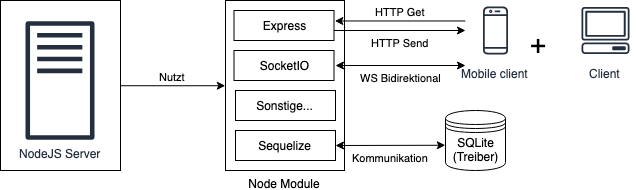
\includegraphics[width=0.8\linewidth]{bilder/server_architektur}
	\caption[Aufbau der geplanten Serverarchitektur]{Aufbau der geplanten Serverarchitektur}
	\label{fig:server_diagram}
\end{figure}
\footnotesize \underline{Hinweis:} NodeJS Module aus der Sektion \textbf{Sonstige Module} wurden aus Gründen der Übersicht in dieser Grafik nicht abgebildet.

\normalsize 
\newpage
\subsection{Entwurf des Clients}\label{sec:clientkonzept}
Wie zuvor in Abschnitt \ref{sec:sysbeschreib} erörtert, ist es vorgesehen drei verschiedene Clients zu implementieren, welche alle auf dem gleichen Prototyp basieren sollen, allerdings verschiedene Zwecke verfolgen. Ein Webclient jeweils für \textbf{Lehrende/Dozierende}, \textbf{Schülerinnen und Schüler} und einen für \textbf{Großbildanzeigen} optimierten wie Projektoren o. Ä. vor. Zur Vereinfachung werden diese gemäß der vorherigen Reihenfolge \textbf{Teacher Client}, \textbf{Student Client} und \textbf{Presenter Client} in diesem und darauffolgendem Kapitel genannt.

\subsubsection{User Interface}\label{sec:uientwurf}
Da das Projekt als Web-Applikation implementiert werden soll, wird das UI gänzlich durch die Stylesheet-Sprache \emph{CSS} beschrieben. Im Jahr 2018 wurden erstmals häufiger mobile Endgeräte wie Smartphones zur Internetnutzung herangezogen als klassische Computer oder Laptops \cite{Rabe2019}. Viele Design-Frameworks setzen daher schon länger auf das Prinzip "`Mobile First"'. Die Applikation soll letztlich sowohl auf Computern und Smartphones aber auch Großbildgeräten angezeigt werden. Ein Web-Design-Framework als Basis, welches bereits viele relevante Web-Design Standards wie das o.g. "`Mobile First"' berücksichtigt, bildet ein solides Fundament in Sachen Usability (Software-Ergonomie) und UI-Design. Eines der populärsten dieser Art ist \emph{Bootstrap}, welches zusammen mit einem frei erhältlichen Design-Theme von \emph{FreeHTML5.co} \cite{FreeHTML5.co2019} genutzt werden soll. Das gewählte Theme soll an die Applikation angepasst und teils für die Großbild Anzeige des Presenter Clients optimiert werden.  
\subsubsection{Browserify}\label{sec:browserify}
Um das Nutzen von NPM Modulen und die damit verbundene \texttt{require()} Funktionalität auch auf der Clientseite zu ermöglichen, soll die Bundle-Soft\-ware~\emph{Brow\-serify}~\cite{Browserify2019} zum Einsatz kommen. Mit ihr können alle Module, welche über den \emph{Node Package Manager} in das Projekt hinzugefügt wurde im Webbrowser des Clients genutzt werden. Dazu bündelt die Bibliothek alle Module und stellt anschließend eine einzige JS-Datei zur Verfügung, die nur noch im HTML-Dokument eingebunden werden muss. Mithilfe der \texttt{require()} Funktionalität, welche eigentlich nur in der \emph{Node.js} Umgebung genutzt werden kann, ist es möglich den Code übersichtlicher in mehrere Dateien/Module aufzuteilen. Dies war früher ohne Aufwand auf der Browser-Seite nicht möglich, ist aber durch die Einführung von Modulen seit ECMAScript\footnote{Der als ECMAScript (ECMA 262) standardisierte Sprachkern von JavaScript beschreibt eine dynamisch typisierte, objektorientierte, aber klassenlose Skriptsprache. (Wikipedia.org)} in Version 6 nun möglich. Oftmals wird aber aus Kompatibilitätsgründen zu älteren Webbrowsern auf Lösungen wie \emph{Browserify} gesetzt. Zusätzlich kann Software wie \emph{Babel} den geschriebenen \emph{JavaScript} Code so übersetzen, dass er auch von älteren Webbrowsern interpretiert wird (auch Transpiler genannt). Sämtliche folglich genannten NPM Module resp. Bibliotheken sollen via \emph{Browserify} in eine \emph{JavaScript} Datei zusammengefasst werden und anschließend pro Client eingebunden werden. Das bringt den zusätzlichen Vorteil, dass für jegliches, auf Browser-Seite eingesetztes JavaScript nur ein einziger HTTP-Get Request für den Code benötigt wird, da wie erwähnt nur eine \emph{JavaScript} Datei pro Client angefordert werden muss. 
\subsubsection{JavaScript Lösungen}\label{sec:clientjs}
Von folgenden JavaScript Lösungen soll auf der Clientseite Gebrauch gemacht werden, um den Implementierungsprozess zu optimieren:
\begin{itemize}
	\item \textbf{VueJS}: Um das Anzeigen, Editieren und Anpassen dynamischer Inhalte zu erleichtern, soll das JS-Webframework \emph{VueJS} \cite{You2019} zum Einsatz kommen, da dieses gut skalierbar ist und alle benötigten Funktionalitäten mit sich bringt. Im Vergleich zu \emph{AngularJS} und \emph{React} (siehe auch Abschnitt \ref{sec:clientseitigeransatz}), biete \emph{VueJS} eine flachere Lernkurve und kann als ein guter Kompromiss aus seinen zwei Konkurrenten betrachtet werden. Mittlerweile hat \emph{VueJS} seinen Konkurrent \emph{React} in Sachen Popularität auf \emph{GitHub} überholt \cite{Daityari2019}. \emph{VueJS} ist auch gemessen an der Dateigröße von nur 80~KB im Vergleich deutlich kleiner als Angular mit 500 KB.
	\item \textbf{Socket.IO}: Das bereits in Abschnitt \ref{sec:socketio} erwähnte \emph{Socket.IO} besitzt ein Bibliotheksteil, welcher auf der Client-Seite im Webbrowser zum Einsatz kommt. Dadurch wird die bidirektionale Kommunikation mit der Server ermöglicht und es soll in beide Richtungen Daten in Echtzeit ausgetauscht werden. 
	\item \textbf{Zingchart}: Zur Visualisierung der Wörterwolke (Word Cloud), welche bei der interaktiven Unterrichtsmethode Brainstorming zum Einsatz kommt, soll die auf diese Szenarien spezialisierte JavaScript Bibliothek \emph{ZingChart} genutzt werden (vgl. Abbildung \ref{fig:wordcloud}). Die Software ist in einer freien Version erhältlich, wobei lediglich stets ein kleines \emph{ZingChart} Logo stets angezeigt wird \cite{zingchartpricing}.
\end{itemize}

\begin{figure}[H]
	\centering
	
\includegraphics[width=0.8\linewidth]{bilder/wordcloud}
	\caption[ZingChart Word-Cloud]{Eine Word-Cloud/Wörterwolke generiert durch ZingChart \cite{ZingSoft2019}}
	\label{fig:wordcloud}
\end{figure}

\subsubsection{Client Architekturdiagramm}\label{sec:clientarchitekt}
Nachfolgend die umzusetzende Architektur der Client-Anwendung. 

\begin{figure}[H]
	\centering
	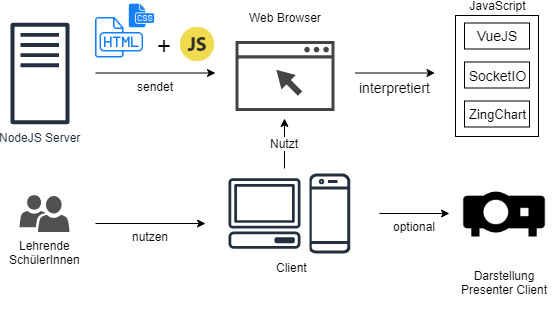
\includegraphics[width=0.8\linewidth]{bilder/client_architektur}
	\caption[Aufbau der geplanten Client Architektur]{Aufbau der geplanten Client Architektur}
	\label{fig:client_diagram}
\end{figure}
\footnotesize \underline{Hinweis:} Zum besseren Verständnis wurden die Rollen des Servers und der Nutzer ebenso dargestellt. Der Presenter Client nutzt in der Grafik ein Projektor. Dies ist eine Option und nicht zwingend von Nöten. Alle Clients können auf dem gleichem Server-Host Computer ausgeführt werden (z.B. in unterschiedlichen Tabs eines Webbrowsers) als auch auf separaten Endgeräten. 



\normalsize

\newpage

\section{Implementierung}\label{sec:implementierung}
%TOTO LEFTOVER: 
%QUIZ
%HTTPS
%WLAN
Das folgende Kapitel wird Einblicke in die Entwicklung der Software im Rahmen des Projekts geben. 
Dabei wird iterativ chronologisch die Vorgehensweise schriftlich reflektiert und an mehreren Stellen 
zum besseren Verständnis auch ein Einblicke in den Sourcecode gegeben. Anknüpfend werden etwaige Probleme bei der Implementierung aufgezeigt sowie mögliche Lösungen diskutiert. 

\subsection{Implementierung der Server-Software}\label{sec:implementserver}
Aufbauend auf das Entwurfs Kapitel soll die Server-Software mit \emph{Node.js} und \emph{Express} als Hauptkomponente entwickelt werden. Dazu wird zunächst im folgenden Abschnitt \ref{sec:implementexpress} der HTTP Server grundlegend konfiguriert und anschließend dessen Routen im darauffolgenden Abschnitt \ref{sec:anlegrouten} angelegt. 

\subsection{ExpressJS Setup}\label{sec:implementexpress}
Nachdem das Projekt grundlegend mit dem Befehl \texttt{npm init} initialisiert wurde,
kann ExpressJS einfach über den \emph{Node Packet Manager} (NPM) hinzugefügt werden. 
Zusätzlich wird das NPM Modul \emph{IP} genutzt um die aktuelle IP-Adresse des Host-Computers automatisch zu ermitteln und
den \emph{Express}-Server auf dieser lauschen zu lassen. Dies wird im folgendem Code-Listing getan:
\begin{lstlisting}[caption=Errichtung des Webservers]
const app = express();
const server = app.listen(3000, server_ip, function () {
logger.log({ level: 'info', message: `Hello! The Server is running on ${server_ip}!`});
});
\end{lstlisting}
Der Server lauscht auf der IP Adresse des Netzwerk-Adapters der Maschine auf dem er ausgeführt wird. Zusätzlich wurde der Port 3000 spezifiziert. Dies kann je nach Konfiguration auf den Standard HTTP Port 80 resp. 443 geändert werden, sollte Verschlüsselung eingerichtet sein (HTTPS).
\\
Anschließend können nun die Routen eingerichtet werden.

\subsection{Autarkes WLAN}\label{sec:eigeneswlan}
Um einen Stand-Alone Betrieb\footnote{Stand-Alone meint einen Betrieb unabhänging von ggf. vorhandenen Netzwerkinfrastruktur am Einsatzort} der Software zu ermöglichen, wird als Lösung der Betrieb eines eigens aufgebautem kabellosen Netzwerkes (WLAN/Wifi) angestrebt. Folgende mögliche Lösungsszenarien wurden ausgearbeitet.
\begin{enumerate}
	\item \textbf{Einfach}: Als einfachste Lösung hat sich der Betrieb eines lokalen WLANs über ein Smartphone oder Laptop herausgestellt. Nahezu jedes Smartphone bzw. jeder Laptop lässt das Generieren eines WLAN Zugangspunktes für andere Geräte zu. Alle Clients und der Server selbst werden mit diesem Netzwerk verbunden. Dies Verbindung wurde getestet und ein Betrieb war möglich. Da hierbei aber auch die Internetverbindung des Zugangspunktes freigegeben wird, was ggf. unerwünscht sein kann, würde es sich anbieten eine spezielle "`Companion App"' zu entwickeln und für \emph{Android} / \emph{iOS} basierte Smartphones zu anzubieten. Diese App könnte automatisch einen WLAN-Hotspot erstellen und den Netzwerkverkehr ins Internet eventuell limitieren. Gleiches gilt analog für windows- oder unixbasierte Computer, ist aber problematischer, siehe dazu nächster Listenpunkt.
	\item \textbf{Speziell}: Um auf einem Computer vollautomatisch einen WLAN Hotspot zu genieren, bedarf es Administrator Privilegien sowie genauere Kenntnisse über den verwendeten Netzwerkadapter. NodeJS selbst bietet nur eingeschränkt Möglichkeiten an, diese Aufgabe autark zu übernehmen, könnte aber ggf. eventuelle Shell-Skripte triggern. Unter \emph{Microsoft Windows 7} und höheren Versionen, gibt es mit den NPM Paket \texttt{node-hotspot} auch die Möglichkeit, dies direkt mit \emph{Node.js} zu erledigen. Dieses Paket wird in die zu entwickelnde Software integriert und soll anschließend unter einer \emph{Microsoft Windows} Umgebung das generieren eines WLAN Hotspots / Zugangspunktes ermöglichen. Zur Verwendung werden entsprechende Steuerungsoptionen in Einstellungsbereich im Lehrkraft Backend integriert. Die interne Steuerung erfolgt über Routen (siehe auch Abschnitt \ref{sec:anlegrouten}).
	
Wird die Applikation in einer vorhandenen Netzwerkinfrastruktur betrieben, ist ein Betrieb in jedem Falle gewährleistet. Ist diese Vorraumsetzung nicht gegeben, könnte ein mobiler WLAN-Router genutzt werden, sollte keine ausreichende Infrastruktur vorhanden sein. Dieser müsste einmalig konfiguriert werden und ist anschließend in der Lage die Serverapplikation für Clients ansprechbar zu machen. Ein solches Gerät gibt es bereits ab ca. 10 Euro zu erwerben.
\end{enumerate} 

\subsection{Verschlüsselung}\label{sec:encrypted}
Um eine verschlüsselte Kommunikation zwischen Server und Clients zu gewährleisten, sollte der Datenaustausch nicht über das HTTP Protokoll,  sondern über das HTTPS Protokoll erfolgen. Um HTTPS allerdings sinnvoll nutzen zu können, ist ein Zertifikat von einer Zertifizierungsstelle (CA) notwendig, was, mit Kosten verbunden ist. Das Zertifikat gewährleistet die Identität des Servers. Allerdings bietet der Anbieter \emph{Let's Encrypt} \cite{LetsEncrypt.org} kostenlose Zertifikate an, welche sich problemlos bei vorhandenem SSH-Zugang installieren lassen. Hier wird aber nur die Domain zertifiziert. Bezahlte Zertifikate von anderen CAs bieten im Vergleich höheren Support und es wird nicht nur die Domain an sich zertifiziert, sondern das ganzen Unternehmen an sich. Außerdem besteht ein Gewährleistungs- und Garantieanspruch gegenüber der CA \cite{Ali2019}. \\
Für den Intranet Betrieb können auch eigens ausgestellte Zertifikate genutzt werden, welche mit Shell-Programmen wie \texttt{openssl} generierbar sind \cite{Copes2018}. Allerdings warnen moderne Webbrowser den Nutzenden recht auffällig, dass die genutzte Verbindung dennoch nicht sicher ist, da dem Zertifikat nicht vertraut werden kann. Soll die Applikation rein im Intranet laufen, könnte die Schule alternativ eine Sub-Domain anlegen, welche nur aus dem Intranet erreichbar ist und ebenfalls durch ein signiertes Zertifikat geschützt ist. \\Der HTTPS Betrieb wurde erfolgreich getestet. Die Implementierung ist nicht aufwendig allerdings, birgt aber den o.g. Nachteil. Da das Intranet ein an sich abgeschlossenes Netzwerk ist, scheint der verschlüsselte Betrieb in diesem zunächst nicht wichtig, kann aber jederzeit realisiert werden und ist bei Betrieb im Internet als obligatorisch zu betrachten. 

\subsection{Anlegen der Routen}\label{sec:anlegrouten}

Grundlegend soll es folgende Routen auf dem Server geben:
\begin{itemize}
	\item \textbf{"`/"'}: Die Haupt Route, sie wird angesteuert, wenn der Server einfach unter seiner IP (oder eingerichteter Domain) kontaktiert wird. Hier wird anschließend die Rolle des Nutzers (Lehrender oder Schülerin/Schüler) abgefragt  und dementsprechend weitergeleitet.
	\item \textbf{"`/teacher"'}: Diese Route verweist auf den Lehrerbereich der Anwendung, man kann sie auch als Backendbereich bezeichnen. Alle hinter dieser Route liegende Routen bedürfen einer Authentifizierung seitens des Nutzenden.
	\item \textbf{"`/client"'}: Diese Route verweist grundlegend auf den Student Client. Aber auch der Presenter Client wird über diese Weiche aufgerufen. 
\end{itemize}
Neben diesen drei Hauptrouten existieren noch weitere Routen für das Error-Handling (z.B. "`404 - Seite nicht gefunden"') sowie besondere für die \emph{WebSocket}-Kommunikation, welche aber im Hintergrund genutzt werden.
Das Anlege der Routen ist mit folgendem Codeausschnitt durchgeführt:
\begin{lstlisting}[caption=Anlegen der Routen]
app.use('/teacher', teacherRoutes);
app.use('/client', clientRoutes);
app.use('/', mainRoutes);
\end{lstlisting}

\footnotesize{Die Route Module werden im Hauptmodul (app.js) referenziert und deren Zuständigkeit festgelegt.} \\ \\
\normalsize
Zu beachten ist: Die weiterführenden Routen werden in Dateien ausgelagert, um die Übersicht des Quelltextes zu wahren. Zudem sind auch diese Routen sog. Middleware-Funktionen. Dies wird im nächsten Abschnitt genauer beleuchtet. Daher ist auch die Reihenfolge wichtig, wie in Listing 2 dargestellt. Würde die \texttt{"`/"'}~Route als erstes angelegt werden, so würde diese alle folgenden, spezifischeren "`abfangen"'.  

\newpage
\subsection{Reflexion des MVC Schemas}\label{sec:mvc}
Da der Server grundlegend nach dem \emph{Model-View-Controller} Muster  arbeiten soll, gilt es dieses zu implementieren. Die folgende Tabelle \ref{tab:mvcschema} gibt einen Überblick über die anfallende Struktur:

\begin{table}[h!]
	\caption{MVC Struktur der Implementierung}
	\label{tab:mvcschema}
	\begin{tabular}{llll}
		
		\multicolumn{1}{c}{\textbf{Betrifft}}                         & \multicolumn{1}{c}{\textbf{Model}} & \multicolumn{1}{c}{\textbf{View(s)}}                                                                         & \multicolumn{1}{c}{\textbf{Controller}}                                            \\ \toprule
		Lehrende                                                        & user.js                             & \begin{tabular}[c]{@{}l@{}}teacher/new.pug\\ teacher/signup.pug\\ teacher/user-edit.pug\end{tabular}          & teacher.js                                                                          \\ \rowcolor[HTML]{EFEFEF} 
		\begin{tabular}[c]{@{}l@{}}Schülerinnen/\\ Schüler\end{tabular} & student.js                          & student.pug                                                                                                   & client.js                                                                           \\ 
		Lehreinheiten                                                   & eduSession.js                       & \begin{tabular}[c]{@{}l@{}}edusessions/*/*.pug\\ edusessions/index.pug\\ edusessions/running.pug\end{tabular} & \begin{tabular}[c]{@{}l@{}}session.js\\ quizzing.js\\ brainstorming.js\end{tabular} \\ \rowcolor[HTML]{EFEFEF} \midrule
	\end{tabular}
\footnotesize {
	\underline{Hinweis:} Zum Zwecke der Übersicht wurden einige interne Controller-Dateien nicht gelistet, wie z.B. der Error-Controller, welcher zwar eine View besitzt, jedoch kein Model. 
}
\end{table}

Nun sollen die entsprechenden Controller-Funktionen an die Routen gebunden werden. Entsprechende Unterrouten werden zu den aus Abschnitt \ref{sec:anlegrouten} bereits angelegten hinzugefügt. Im Sinne der Übersicht wird hierzu ein Routen-Ordner angelegt, welcher Routen-Module enthalten soll. 
Folgende Routen-Module werden angelegt: \\ \\
\textbf{routes/main.js}: Generelle Routen (Startseite etc.). \\
\textbf{routes/client.js}: Student Client / Presenter Client relevanten Routen.\\
\textbf{routes/teacher.js}: Alle für das Backend resp. Lehrerbereich relevanten Routen.\\ \\
Es folgt ein Codebeispiel (Listing 3) aus der Datei \texttt{routes/client.js}. 
\begin{lstlisting}[caption=Unterrouten und Controlleranbindung]
// 3rd Party Imports
const express = require('express');
const router = express.Router();
// App Imports
const clientController = require('../controllers/client');
const isAuth = require('../middleware/is-auth');
// Presenter & Student Clients
router.get('/presenter/:sessionId', isAuth, clientController.getPresenter);
router.get('/student', clientController.getStudent);
router.get('/', clientController.getStudent);
module.exports = router;
\end{lstlisting}
\newpage
Zur Verdeutlichung wird anknüpfend die in Zeile 10 des vorangegangen Listings 3, die Funktion \texttt{getStudent} des Controllers in Listing 4 gezeigt:
\begin{lstlisting}[caption=GET Funktion des Student Controllers]
// GET => /client/student
exports.getStudent = (req, res, next) => {

return res.render('client/student',
	{
		docTitle: 'Student | Node ICT',
		ipAdd: ip.address(),
	});
};
\end{lstlisting}
 
 \subsection{Einrichtung der Datenbank}
 Die SQL Datenbank \emph{SQLite}  und der Object-Relationship-Mapper \emph{Sequelize} können unkompliziert über NPM dem Projekt hinzugefügt werden.  
 Nach diesem Schritt kann die Anbindung und Einpflegung folgen. Hierzu wird ein Datenbank Utility Modul angelegt, dieses soll die grundlegende Konfiguration der Datenbank enthalten und ausführen. All dies kann direkt über \emph{Sequelize} erfolgen, welches im Hintergrund die notwendigen Schritte vornimmt. Der Dialekt \texttt{sqlite} muss in der \emph{Sequelize} Konfiguration angegeben werden sowie der Pfad unter welchem die Datenbank als Datei gespeichert werden soll. Gemäß dem logischen Aufbau einer SQL Datenbank folgt nun das Konfigurieren und Anlegen der Tabellen und deren Beziehung untereinander. Dieser Arbeitsschritt erfolgt relativ intuitiv. Im folgenden Code-Listing 5  wird die Tabelle bzw. das \emph{Sequelize}-Model "`student"' im Modul \texttt{tables} konfiguriert.
 
 \begin{lstlisting}[caption=Anlegen einer Tabelle und deren Beziehungen]
exports.student = (sequelize, Sequelize) => {
	return sequelize.define('student', {
		id: {
			type: Sequelize.INTEGER,
			autoIncrement: true,
			allowNull: false,
			primaryKey: true
		},
		name: {
			type: Sequelize.STRING,
			allowNull: false
		},
	})};
 \end{lstlisting}
 Im Datenbank Modul \texttt{util/database.js} wird nun die Konfiguration geladen und anschließend dessen Beziehung zu anderen Entitäten eingestellt. Durch \emph{Sequelize} kann hier ein relativ natürliches Sprachbild verwendet werden. Das folgende Code-Listing 6 zeigt die Beziehungen zwischen \texttt{EduSession} und \texttt{Student} an:
 \begin{lstlisting}[caption=Konfiguration von Entitätsbeziehungen]
 EduSession.hasMany(Student, { onDelete: 'cascade' });
 Student.belongsTo(EduSession);
 \end{lstlisting}
 Nach demselben Schema werden nun für alle Modelle entsprechende Tabelle angelegt und deren Beziehungen untereinander festgelegt. 
 \paragraph{Datenbank Interaktion}
 Um Datenbank Anfragen (Queries) zu stellen, bietet \emph{Sequelize} viele Optionen an. Diese müssen nicht in SQL geschrieben werden, sondern sind normale JS Funktionen. Jedes innerhalb \emph{Sequelize} definierte Model bietet diese automatisch an. Als Beispiel könnte nun über den JS Code 
 \texttt{const~studentToFind~=~await~Student.findByPk(1);} die Entität mit der ID~1 aus der Datenbank geladen werden. All diese bereitgestellten Funktionen sind \emph{JavaScript Promises}, d.h. sie werden asynchron ausgeführt auch nicht erfüllen des \emph{Promise} gilt es zu berücksichtigen.
 Im Erfolgsfall befindet sich in der Variabel nun das Objekt der Entität und dieses bietet wiederum Funktionen zur Interaktion an. Eine ausführliche Dokumentation findet sich auf der Webpräsenz von~\emph{\-Sequelize}~\cite{Depold2019}. 
 Die in Tabelle \ref{tab:mvcschema} gelisteten Models werden gemäß der Arbeitsteilung des MVC-Schemas hauptsächlich direkt mit \emph{Sequelize} arbeiten und den Controllern entsprechende Funktionen bereitstellen.
 \subsection{Implementierung des Lehrer-Bereiches}\label{sec:implementlehrer}
 %hier halt sessions zum einlogge
 % Das Grundsetup wenn alles neu
 % User Anlegen / Freischalte / Sicherheit bei der Datenfreigabe 
 % Anlegen von Lehreinheiten + Brainstorming + Quizzing
 Nachdem die aus Abschnitt \ref{sec:mvc} genannten Models angelegt wurden, welche direkt mit der Datenbank interagieren, müssen anschließend Controller für die verschiedenen Abschnitte des Webservers implementiert werden. Jedes Model hat dabei einen zugehörigen Controller, welcher entsprechende Funktionen für die Routen exportiert. Wie in Listing 3 beispielhaft zu sehen, wird die GET-Route "`/student"' mit der nach außen hin exportierten Funktion \texttt{getStudent} assoziiert. Um eine einheitliche Struktur zu gewährleisten, werden exportierte Funktionen eines Controller Moduls immer nach der jeweilig bedienten Request-Methode benannt \\(GET, POST, etc.).
 \newpage
 \paragraph{View Rendering mit Pug}
Für alle Views soll die Template-Engine \emph{Pug} zum Einsatz kommen (siehe auch Kapitel \ref{sec:konzept} Konzept). Dazu wird \emph{Pug} für das Rendern aller HTML-Dokumenten, welche nicht statischen Routen zugehörig sind, im Hauptmodul der Software registriert. \emph{Pug} macht das Schreiben von HTML Dokumenten sehr komfortable und unterstützt Vererbung (Layouting). So wird zunächst für den Lehrer-Bereich ein Haupt-Layout angelegt, von dem später alle anderen, diesem Bereich zugehörigen Views, erben. Die Layouts können zusätzlich so genannte Blöcke enthalten, welche später dann dynamisch mit Inhalten gefüllt werden. Die Controller können Daten an die Views übergeben, welche von diesen dann dargestellt werden. 

Dazu bietet \emph{Pug }Funktionen wie das Iterieren über Datensätze mittels Schleifen an. Auch dynamisch generierte Inhalte, abhängig von konditionalen Ausdrücken, sind möglich. Sämtliche an die Clients ausgelieferte HTML Dokumente sollen von \emph{Pug} "`on-demand"' generiert werden. \emph{Pug} benutzt seine eigene \emph{Templating-Language}, welche sich deutlich von HTML unterscheidet, aber sehr intuitiv und schnell zu lernen ist. So wird die Hierarchie der HTML Elemente allein durch Einrückung bestimmt. Somit entfällt das Schließen dieser komplett. Siehe hierzu Abbildung \ref{fig:pug}. \\

\begin{figure}[h!]
	\centering
	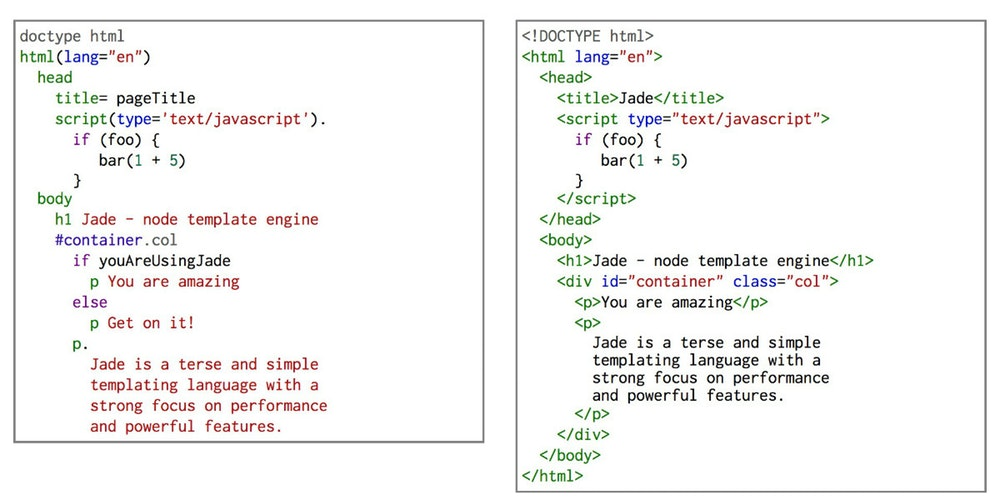
\includegraphics[width=1\linewidth]{bilder/pug}
	\caption[Pug im Vergleich zu HTML]{Pug im Vergleich zu HTML \cite{Janschltz2015}:\\Rechts abgebildet \texttt{Pug}, Links \texttt{HTLM}. Durch die Einrückung und dem Wegfall von schließenden Tags ist der Code deutlich übersichtlicher.}
	\label{fig:pug}
\end{figure}


 
Es werden anschließend für alle Models Views angelegt, damit Lehrende sich anmelden und einloggen, sowie neue Benutzer anlegen und editieren können. Ebenso für das Erstellen von Lehreinheiten mit den Unterrichtsmethoden Brainstorming und Quiz. Dabei werden bei Dateneingabe HTML-Formulare verwendet, welche anschließend via POST-Request an den Server geschickt werden. Controller validieren und werten diese folglich aus. Die Implementierung für das tatsächliche Ausführen der Unterrichtsmethoden wird in Abschnitt \ref{sec:implementclients} beschrieben. 

\subsection{UI Design}\label{sec:uidesign}
Aufbauend auf den Abschnitt \ref{sec:uientwurf} des Entwurf-Kapitels wird zur Designumsetzung das Frontend-CSS-Webframework \emph{Bootstrap} \cite{Twitter2019} genutzt. Dieses kann ebenfalls einfach über NPM dem Projekt hinzugefügt werden. Als Design-Theme bildet das frei erhältliche \emph{Bootstrap}-Theme \texttt{Neat} von \emph{freehtml5.co} die Grundlage (siehe Abbildung \ref{fig:screenshot_lehreinheiten}). Dieses wird hauptsächlich im Lehrerbereiches genutzt und in angepasster Version für den Student Client und den Presenter Client. Letzterer wird insbesondere für die Nutzung auf Großbildgeräten wie Fernsehern und Projektoren optimiert. Es wird sichergestellt, dass sich die Software angenehm auf stationären wie mobilen Endgeräten nutzen lässt. 

\begin{figure}[h!]
	\centering
	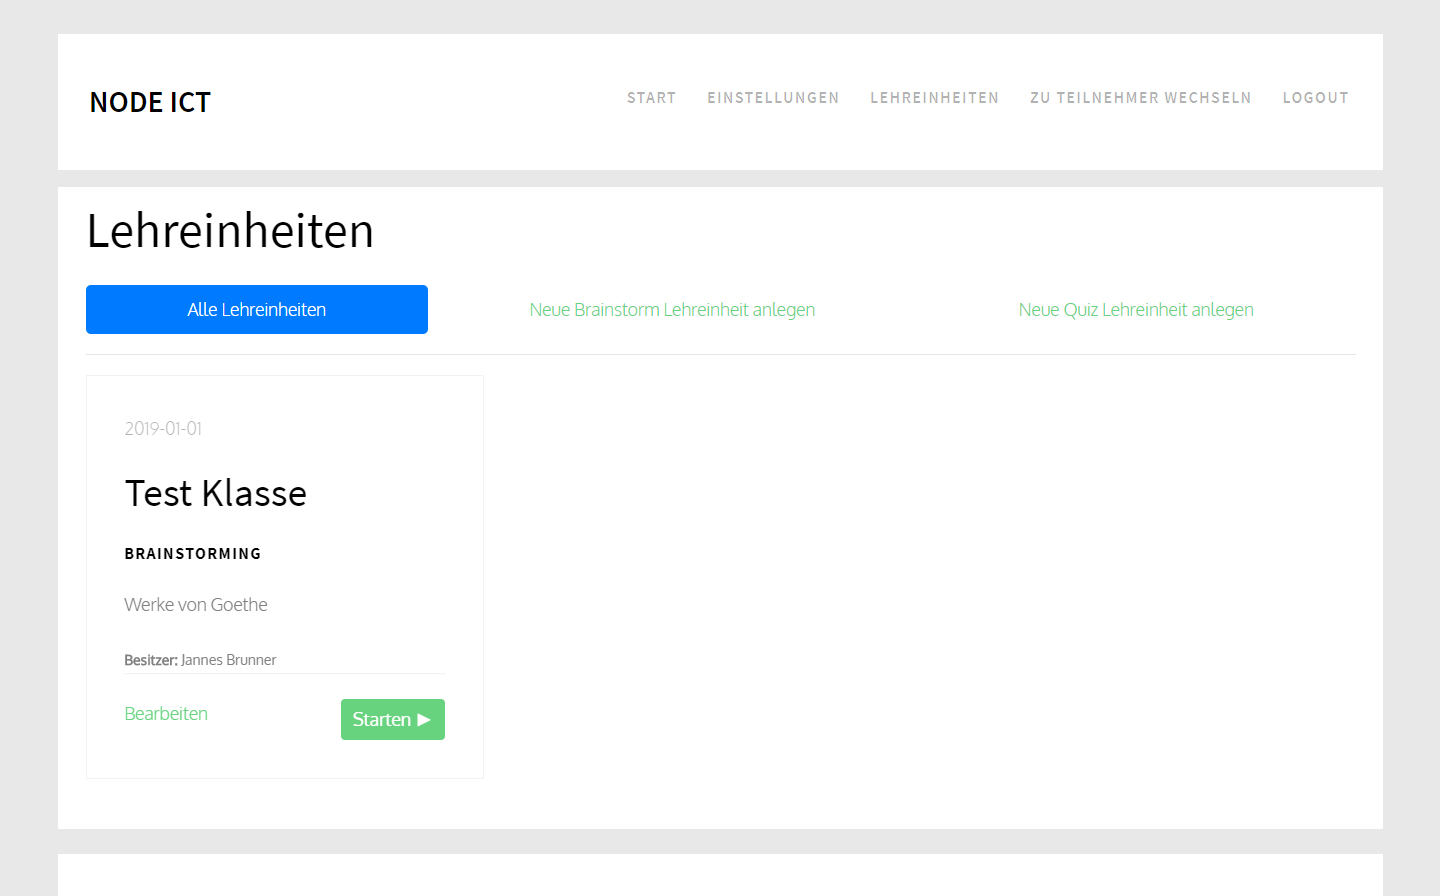
\includegraphics[width=0.9\linewidth]{bilder/screenshot_lehreinheiten}
	\caption[Screenshot UI Design Lehreinheitenbereich]{UI Design der Applikation beispielhaft illustriert durch ein Screenshot des Lehreinheiten Bereiches im Backend Zugang des Teacher Clients.}
	\label{fig:screenshot_lehreinheiten}
\end{figure}

\paragraph{Absicherung des Bereiches}
Bestimmte Bereiche der Applikation sollen nur registrierten und freigeschalteten Benutzenden zugänglich sein. Beim erstmaligen Initialisieren wird der Server mit einem Super-Administrator Account eingerichtet. Nur dieser soll neue Nutzer freischalten, andere Lehrende zu Administratoren ernennen und die Applikation auf Werkseinstellungen zurücksetzen können. Eine entsprechende Einrichtungsmaske soll beim ersten Serverstart automatisch erscheinen. Um dies technisch zu realisieren, wird das aus dem Kapitel \ref{sec:konzept} genannte \texttt{express-session} NPM-Modul genutzt, welches bereits vollständig mit der von \emph{Sequelize} verwalteten \emph{SQLite} Datenbank kompatibel ist. Nach der Einrichtung im Hauptmodul wird eine eigene Middleware-Funktion geschrieben, welche bei allen abgesicherten Routen als erstes aufgerufen wird und überprüft, ob die vom Client übertragene Session noch gültig ist.
\begin{lstlisting}[caption=Code der Authentifizierungs Middleware]
module.exports = (req, res, next) => {
	if(!req.session.isLoggedIn) return res.redirect('/teacher/login');
	next();
}
\end{lstlisting}
Falls dies nicht der Fall ist, wird auf die Login Seite verwiesen. 
Das Verwalten der Sessions und das Generieren von Cookies für die Client-Seite wird automatisch von dem Modul übernommen.
 \subsection{Umsetzung des Client Softwareanteile}\label{sec:implementclients}
 %Hier auch setup, browserify! 
 % vuejs, etc pp
Nachdem die Funktionen "`Erste Initialisierung der Software"', "`Login/Logout"' inkl. Benutzerverwaltung sowie das Anlegen und Verwalten von Lehreinheiten des Typs Brainstorming und Quiz implementiert sind, sollen die Lehreinheiten auch aktiv ausgeführt werden können. Dies bildet die Kernfunktion der Software und verlangt mehr Interaktion auf der Client Seite.\\ \\ 
\emph{Browserify} wird einfach über NPM dem Projekt hinzugefügt und ist anschließend einsatzbereit. Alle im Abschnitt \ref{sec:clientjs} des Kapitels Konzept erwähnten JS-Lösungen sind als NPM Modul verfügbar und werden ebenfalls dem Projekt hinzugefügt. Pro Client (Teacher Client, Student Client, Presenter Client) wird ein Development-Modul angelegt (\texttt{dev.js}). In diesem können alle benötigten JS-Bibliotheken normal importiert und genutzt werden. 
Via \emph{Browserify} wird anschließend pro Client ein Production-Modul generiert (index.js), welches alle notwendigen Importe bündelt. Um diesen Prozess zu automatisieren, wird ein Skript erstellt, welches vom NPM ausgeführt werden kann. Nur das Production-Modul muss via \texttt{script}-tag in das jeweilige \emph{Pug} Template pro Client eingebunden werden. Dies reduziert gleichzeitig die Anzahl notwendiger GET-Requests auf der Client-Seite. \\
Pro Client wird die UI mit dem JS-Framework \emph{Vue.js} kontrolliert und verwaltet. 
Auf dem HTML Layout wird ein \texttt{div}-Element als Ankerpunkt definiert und alle unterliegenden Elemente stehen fortan zur dynamischen Anpassung bereit. Mittels Datenbindung (Data-Binding) hält \emph{Vue.js} die angezeigten Informationen auf dem UI aktuell. \emph{Vue.js} ist dabei pro Client als einfaches JS Objekt auch von außen ansprechbar, was die Schnittstelle für andere Bibliotheken, insbesondere \emph{Socket.IO}, bildet. \emph{Socket.IO} auf der Client-Seite ist für den gesamten Datenverkehr zwischen Server und Client verantwortlich. Sowohl auf Server- wie auch Client-Seite können sog. "`Listener"' programmiert werden, die auf bestimmte Ereignisse (Events) von der, jeweils anderen Seite ausgelöst, lauschen. Im Ereignisfall wird eine anonyme Funktion aufgerufen, welche sich um die eintreffenden Daten kümmert. Die ausgetauschten Daten müssen hierbei nicht zwangsläufig zuvor in das  JSON-Format umgewandelt werden, wie dies sonst bei REST-Apis üblich ist. \\ \\ Auf der Server-Seite kümmert sich das Modul \texttt{ioSocketHandler.js} um alle eingehend Web-Socket Verbindungen und ordnet diesen zunächst einem Namensraum (Name\-space) zu. Ein Student Client wird dabei immer dem Namensraum für Student Clients zugeordnet und steht als Socket Objekt zur Verfügung, übliche Clients diesem Schema folgend.  Nach erfolgreicher Verbindung wird dem Student Client eine Liste verfügbarer Lehreinheiten geschickt und diesem auf der Client Seite dargestellt. Pro Lehreinheit (Typ Brainstorming oder Quiz) gibt es einen "`Session Handler"', der als JavaScript Klasse implementiert ist. Startet eine Lehrkraft eine Lehreinheit wird abhängig vom Typ eine neuen Klasseninstanz angelegt und eine Referenz in einem Speicher gehalten. Tritt nun ein Schüler der Lehreinheit bei, übergibt das übergeordnete "``Socket Handler"'-Modul das Socket-Objekt der Klasseninstanz der Lehreinheit. Die gesamte Logik und Kommunikation der auszuführenden Lehreinheit wird von der jeweiligen Klasse übernommen. Beendet eine Lehrkraft die Session, wird diese aus dem Speicher entfernt und steht nicht mehr zum Beitreten zur Verfügung. Pro gestartete Session kann über einen speziellen Link der passende Presenter Client aufgerufen werden. Dieser wird ebenfalls über das \texttt{ioSocketHandler.js} Modul der jeweiligen Klasseninstanz zugeordnet. Im Listing 8 wird ein Codeauszug gezeigt, welcher den Datenaustausch zwischen Server und Client zeigt.
\begin{lstlisting}[caption=Server Socket Event-Emitierung]
/// TEACHER :::::::
updateSessionT() {
	this.socketT.emit("updateSession", this.session);
}
\end{lstlisting}

Der Server schickt das Event \texttt{updateSession} an den Teacher Client.
Als Inhalt der Nachricht wird das Session Objekt (\texttt{this.session}) übermittelt.
\begin{lstlisting}[caption=Client Socket Event-Listener]
// Sever tells client to update the session object
socket.on("updateSession", function (newSession) {
	console.log("getting fresh session from server...", newSession)
	if (newSession && newSession.id == vue.session.id) {
		vue.session = newSession;
	}});
\end{lstlisting}

Der Teacher Client lauscht auf das Event \texttt{updateSession}. Trifft dieses ein,
wird eine anonyme Funktion aufgerufen, welche sich dem Inhalt der Nachricht annimmt.
Diese überprüft in diesem Fall zunächst, ob sich die ID des zu aktualisierenden Session Objekts
mit dem ursprünglichen deckt. Anschließend wird das alte Session Objekt auf das neue referenziert.  
 
\subsection{Herausforderungen der Implementierung}\label{sec:probsserver}
%ioSessionHandler Socket Handling
%Word Cloud passende finden und praktikabel 
%Wifi Hotspot node module 
%Allgemeiner Umfang von VueJS und sein Einsatz
Während der Implementierung stellte sich anfangs das Verbindungsmanagement der verbundenen Clients über \emph{Socket.IO} als instabil heraus, da Sockets sich bei Verbindungsabbruch zwar selbständig erneut verbinden, jedoch immer unter einer neuen Session ID. Dies führte zunächst zu unerwartetem Verhalten während einer Lehreinheiten Ausführung. Dem konnte aber durch zusätzliche Authentifizierungsdaten entgegengewirkt werden. Bei mobilen Geräten wie Smartphones erwies sich der Verbindungsabbruch zusätzlich als geräteabhängig. Manchen Geräten unterbrechen die Verbindung z.B. beim Ausschalten des Bildschirms sofort, während andere diese im Hintergrund weiterhin aufrecht erhalten. \\ Außerdem war es schwierig ein gut funktionales "`Word-Cloud / Wörterwolke"'-Modul zu finden, welches sich ohne nennenswerte Probleme mit \emph{Vue.js} im Einklang nutzen lassen konnte. Generell wird \emph{Vue.js} in diesem Projekt recht rudimentär eingesetzt, was seine Funktionsweise zwar nicht einschränkt, jedoch das volle Potential dieser Web-Frontend-Engine nicht gänzlich nutzt. \\ \\ Das NPM-Modul \texttt{node-hotspot} wurde zwar gemäß der Instruktionen der Entwickler implementiert, allerdings konnte auf mehreren \emph{Microsoft Windows} Testsystemen nicht selbstständig ein WLAN-Hotspot aktiviert werden. Leider war \texttt{node-hotspot} zum Entwicklungszeitpunkt (Stand Juli 2019) das einzige verfügbare NPM-Modul, welches die Generierung eines WLAN-Hotspots bezweckte. 
 
 
 
\newpage


\section{Auswertung}\label{sec:auswertung}
\newpage

\section{Ausblick}\label{sec:ausblick}
%electron!
%  Eine hier angesetzte Refaktorierung ist vuejs und socketIO
% REST statt Sockets
% 
\subsection{Optimierungspunkte der Software}\label{sec:opti}
Der Nachrichtenaustausch, welcher über das \emph{WebSocket} Protokoll via \emph{Socket.IO} realisiert ist, sollte mehr vereinheitlicht werden. Grundsätzlich lassen sich jede Art von \emph{JavaScript} Daten übertragen; ein strengeres Konzept kann hier das Verständnis für andere Entwickler fördern und den Code sauberer halten. Gerade der Ausführungscode der interaktiven Unterrichtsmethoden könnte noch besser gekapselt und noch sinnvoller aufgeteilt werden, auch in Hinblick auf die Daten, welche zwischen Server und Client ausgetauscht werden. Der Installationsprozess könnte ggf. noch automatisierter erfolgen und so wenig Technik affinen Nutzenden die Installation erleichtern.   
Der Code der Web-Clients, welcher im Webbrowser ausgeführt wird, kann mit mehr Kenntnissen über die Entwicklung mit \emph{Vue.js} und \emph{Socket.IO} optimiert werden. 
\subsection{Anknüpfende Ansätze}\label{sec:ansatze}
Das Projekt soll zukünftig weiterhin ausgebaut werden. Während der Entwicklung kamen immer wieder Ideen für weitere Funktionen auf, welche aber aus Gründen der Priorität nicht implementiert worden sind oder nur als Konzept vorlagen. Dies wären z.B. Funktionen, die den Dozierenden noch intensiver während des Unterrichts unterstützen oder das Schreiben einer API, um die Software an andere Systeme anbinden zu können. Zum Zeitpunkt des Abschlusses des Projekts kann eine Lehrkraft ein Lehreinheit anlegen, welche eine Unterrichtsmethode (Brainstorming oder Quiz) beinhalten kann. Die Umsetzung weiterer Unterrichtsmethoden wäre wünschenswert. Ebenso die Option, dass eine Lehreinheit mehrere Unterrichtsmethoden beinhalten kann. Ein weiteres Vorhaben wäre es, die Software in einem \emph{Fork} nach dem REST-Design aufzubauen und die Kommunikation dementsprechend umzugestalten, um anschließend zu vergleichen, welche Vorgehensweise entsprechende Vor- und Nachteile mit sich bringt. \\ Die Entwicklung einer Desktop-Applikation wäre dank der 
\emph{Node.js} Basis des Projekts mit dem Framework \emph{Electron} realisierbar.
\newpage





%\fancyhead[L]{\textsl{\small \leftmark}}
%\input{sections/07Zusammenfassung.tex}%\newpage
%\input{sections/08Ausblick.tex}\newpage

%\addcontentsline{toc}{section}{Literaturverzeichnis}
%\printbibliography[nottype=online, title={Literaturverzeichnis}]
%\printbibliography[type=online,title={Online - Bildquellen}]\newpage

\printbibliography[title={Literaturverzeichnis}]
\newpage


\addcontentsline{toc}{section}{Abbildungsverzeichnis}
\listoffigures\newpage
\addcontentsline{toc}{section}{Tabellenverzeichnis}
\listoftables
\addcontentsline{toc}{section}{Listingverzeichnis}
\lstlistoflistings
%\clearpage%\vspace*{-3cm}
\newpage

\addcontentsline{toc}{part}{Anhang}

\fancyhead[L]{\textsl{\small \leftmark \hspace{0.8cm}\rightmark}}

\appendix
\thispagestyle{empty}
\part*{Anhang}
\subsection*{Abschnitt: Funktionale Anforderungen}

\begin{table}[h!]
	\caption{Funktionale Anforderungen an die Projektsoftware}
	\label{tab:funkanf}
	\resizebox{\textwidth}{!}{%
		% Please add the following required packages to your document preamble:
		% \usepackage{booktabs}
		% \usepackage[table,xcdraw]{xcolor}
		% If you use beamer only pass "xcolor=table" option, i.e. \documentclass[xcolor=table]{beamer}
		\begin{tabular}{@{}cllc@{}}
			
			\toprule
			\rowcolor[HTML]{FFFFFF} 
			\textbf{ID} & \multicolumn{1}{c}{\cellcolor[HTML]{FFFFFF}\textbf{Name}} & \multicolumn{1}{c}{\cellcolor[HTML]{FFFFFF}\textbf{Beschreibung}}                                                                                                                                                                                                                                                                 & \textbf{Status} \\ \midrule
			\rowcolor[HTML]{FFFFFF} 
			F01         & Datenbankanbindung                                        & Es soll erfolgreich eine Anbindung an die Datenbank erfolgen                                                                                                                                                                                                                                                                      & OK              \\
			\rowcolor[HTML]{EFEFEF} 
			F02         & Datenbank Generierung                                     & \begin{tabular}[c]{@{}l@{}}Alle nötigen Modelle und Tabellen soll in der Datenbank\\ abgebildet werden und bei bedarf gänzlich neu generiert werden\end{tabular}                                                                                                                                                                  & OK              \\
			\rowcolor[HTML]{FFFFFF} 
			F03         & GET Requests                                              & \begin{tabular}[c]{@{}l@{}}Der Server soll in der Lage sein GET Requests entgegenzunehmen\\ und zu beantworten. Im Fehlerfall soll auch eine Antwort erfolgen.\end{tabular}                                                                                                                                                       & OK              \\
			\rowcolor[HTML]{EFEFEF} 
			F04         & POST Requests                                             & \begin{tabular}[c]{@{}l@{}}Der Server soll in der Lage sein POST Requests entgegenzunehmen\\ und zu beantworten. Im Fehlerfall soll auch eine Antwort erfolgen.\end{tabular}                                                                                                                                                      & OK              \\
			\rowcolor[HTML]{FFFFFF} 
			F05         & Login System                                              & \begin{tabular}[c]{@{}l@{}}Nutzende der Software in der Rolle als Lehrkraft oder Administrator\\ sollen in der Lage sein sich bei dem System mittels Authentifizierung\\ an- und abzumelden mittels HTTP-Session und Session-Cookies\end{tabular}                                                                                 & OK              \\
			\rowcolor[HTML]{EFEFEF} 
			F06         & MVC - Pattern                                             & \begin{tabular}[c]{@{}l@{}}Das Model-View-Controller Muster soll beim Datenfluss im Backend/\\ Lehrerbereich des Servers reflektiert und zum Einsatz kommen\end{tabular}                                                                                                                                                          & OK              \\
			\rowcolor[HTML]{FFFFFF} 
			F07         & WebSockets                                                & \begin{tabular}[c]{@{}l@{}}Bei der Ausführung von Lehreineheiten und den damit verbundenen\\ Unterrichtsmethoden soll die Kommunikation zwischen \\ Server und Web-Client über das WebSocket Protokoll erfolgen\end{tabular}                                                                                                      & OK              \\
			\rowcolor[HTML]{EFEFEF} 
			F08         & Drei Client Implementierung                               & \begin{tabular}[c]{@{}l@{}}Um die Software größtmöglichst flexibel einsetzen zu können, sollen\\ drei verschieden optimierte Web-Clients implementiert werden, genauer\\ einen für die ausführende Lehrkraft, einen für Studierende, eine für \\ Anzeigemedien, auf größere Darstellung optimiert im Unterrichtsraum\end{tabular} & OK              \\
			\rowcolor[HTML]{FFFFFF} 
			F09         & Administration                                            & \begin{tabular}[c]{@{}l@{}}Authentifizierte Nutzer wie Dozierende und Administratoren sollen \\ die Software verwalten können, dies umfasst u.A. das Anlegen und \\ Freischalten von Nutzenden und das Setzen der Werkseinstellungen\end{tabular}                                                                                 & OK              \\
			\rowcolor[HTML]{EFEFEF} 
			F10         & Absicherung                                               & \begin{tabular}[c]{@{}l@{}}Alle Routen die höhere Privilegien verlangen, sollen nur authentifizierten\\ Nutzenden zugänglich gemacht werden, dies betrifft vor allem F09 und\\ Besitzer abhängig erstellte Ressourcen\end{tabular}                                                                                                & OK              \\
			\rowcolor[HTML]{FFFFFF} 
			F11         & Ausführung von Lehreinheiten                              & \begin{tabular}[c]{@{}l@{}}Lehrkräften bzw. Dozierende soll es möglich sein zwei Typen von\\ interaktiven Unterrichtsmethoden mit Studierenden durchzuführen, \\ dies umfasst zunächst die Typen Brainstorming und Quiz\end{tabular}                                                                                              & OK              \\
			\rowcolor[HTML]{EFEFEF} 
			F12         & Einfacher Studierendenzugang                              & \begin{tabular}[c]{@{}l@{}}Studierende bzw. Schülerinnen und Schüler sollen über einen QR Code\\ vereinfacht Zugriff auf den Server erhalten, vorausgesetzt sie sind mit \\ dem gleichem Netzwerk wie der Server verbunden\end{tabular}                                                                                           & OK              \\
			\rowcolor[HTML]{FFFFFF} 
			F13         & Wifi/WLAN Hotspot                                         & \begin{tabular}[c]{@{}l@{}}Der Server soll ein eigenes WLAN Netzwerk bereitstellen können in \\ dem der Host-Computer des Servers als WLAN Access Point fungiert, \\ und verbundenen Clients automatisch eine IP-Adresse zuweist (DHCP)\end{tabular}                                                                              & N.I.*        \\ \bottomrule
		\end{tabular}
	}
	\footnotesize * nicht implementiert
\end{table}
%\input{anhang/Nachmessung_Zemente}

\newpage
\thispagestyle{empty}
\section*{Selbstständigkeitserklärung}\label{sec:selbststandigkeitserklarung}
Ich erkläre hiermit, dass ich die vorliegende Bachelorarbeit selbstständig verfasst und dazu  keine  anderen  als  die  angeführten  Behelfe  verwendet,  die  Autorenschaft  eines Textes  nicht  angemaßt  und  wissenschaftliche  Texte  oder  Daten  nicht  unbefugt verwertet habe. Die elektronische Kopie ist mit den gedruckten Exemplaren identisch.
\vspace{5cm}
\\

Berlin, 05. August 2019, 
\begin{flushleft}
	\line(1,0){350}\\
	(Ort, Datum, Unterschrift)
\end{flushleft}
\thispagestyle{empty}
\end{document}
